
%     Subgigahertzový transceiver
% notes:
%~~~~~~~~~
%---------------------------------------------------------------------------------------------------
% Setting path to image 
\graphicspath{{../src/MOL/img/}}
%---------------------------------------------------------------------------------------------------
% file EXP001.tex
%==================== Kapitola: Subgigahertzový transceiver ========================================

\sisetup{
list-final-separator = { \translate{and} },
list-pair-separator = { \translate{and} },
range-phrase = { \translate{to (numerical range)} },
}


\chapter{Sub-1GHz transciever s obvodem SPIRIT1}
\minitoc
\newpage
  \section{Zadání}
    Postavme nízkopříkonový transceiver vhodný pro bezdrátový přenos dat na velké vzdálenosti mezi 
    řídicím systémem (embedded PC) a senzory. Parametry jsou následující:
    \begin{itemize}\addtolength{\itemsep}{-0.5\baselineskip}
      \item frekvence \SI{468}{\MHz}  
      \item vzdálenost \SI{2000}{\meter} 
    \end{itemize}
    
    \begin{note}
      Pro efektivní řešení úloh tohoto typu je na trhu k dispozici mnoho integrovaných obvodů pro 
      bezdrátový přenos relativně malého objemu dat (řádově desítek kilobytů za sekundu) na 
      vzdálenost až 10 km ve volném prostoru, což je umožněno díky použití subgigahertzového pásma 
      a vysokou citlivostí přijímače (běžně dosahuje -100 dBm). Společně s nízkým příkonem jsou 
      tyto obvody vhodnými kandidáty pro komunikaci mezi různými senzory a regulátory například v 
      budovách, infrastruktuře a v neposlední řadě také pro průmyslové monitorování a řízení 
      využívající bateriové či solární napájení. Vzájemná komunikace jednotlivých zařízení pak 
      tvoří základ nového trendu tzv. Internetu věcí (\texttt{IoT} - \emph{Internet of Thing}). 
    \end{note}
    
  \section{Popis obvodu SPIRIT1}
    Transceiver Spirit1 od STMicroelectronic, který byl pro toto řešení vybrán umožňuje provoz v 
    bezlicenčním pásmu ISM\footnote{Pod pojmem bezlicenční (volné) pásmo se rozumí pásmo kmitočtů, 
    ve kterém je povolen radiový provoz bez licenčních poplatků držitelům homologovaných zařízení, 
    přičemž jejich počet není předem omezen. Tito provozovatelé pak mohou sdílet při provozu celé 
    vyčleněné pásmo, ovšem bez nároku na ochranu proti rušení.} (\emph{Industrial, scientific and 
    medical radio bands}) na frekvencích 169, 315, 433, 868 915 a 920 MHz a navíc dovoluje 
    programově měnit frekvenci ve čtyřech pásmech 150-174 MHz, 300-348 MHz, 387-470 MHz, 779-956 
    MHz. %\SIrange{10}{30}{\MHz}
    
    Jelikož zařízení v pásmu \texttt{ISM} spadají do kategorie \texttt{SRD} (\emph{Short Range 
    Devices}) tj. zařízení krátkého dosahu, mají vysílače omezený výkon na 25 až 100 mW efektivního 
    vyzářeného výkonu (ERP). Obvod \texttt{Spirit1} v tomto směru nabízí programové řízení 
    výstupního výkonu do maximální hodnoty +16 dBm (40 mW). Přenosová rychlost je volitelná od 1 do 
    500 kbps, odstup kanálu lze vybírat v souladu s normou EN 300 220 mezi 12.5/25 kHz.
    
    Z programátorského hlediska je důležité, že obvod má konfigurovatelný datový management, 
    umožňující tvorbu vlastního paketového formátu, acknowledgement, retransmission, and timeout 
    protocol engine. K dispozici je také CSMA/CA engine. Data lze implicitně kontrolovat pomocí CRC 
    nebo lze  použít FEC encoding/decoding pro pakety. Pro zabečený přenos dat je možné využít 
    128-bitový kryptovací engine. Přijímaná i vysílaná data jsou ukládána do vlastní vyrovnávací 
    paměti typu \texttt{FIFO}\footnote{(\texttt{TX FIFO} a \texttt{RX FIFO})}. Obě paměti jsou  
    dostupné přes \texttt{SPI} rozhraní.

    Souhrn Klíčových vlastností transceiveru Spirit1:
      \begin{itemize}\addtolength{\itemsep}{-0.5\baselineskip}
        \item Frequency bands: 169, 315, 433, 868, 915, 920 MHz
        \item Configurable data rate from 1 to 500 kbps
        \item SPI, GPIO interface
        \item Supply voltage: 1.8 V to 3.6V
        \item Modulation schemes: 2-FSK, GFSK, MSK, GMSK, OOK, ASK  
        \item Output Power: -36 dBm to +11 dBm (16dBm in boost mode)
        \item Receiver sensitivity: 
          \begin{itemize}
            \item -123 dBm (1.2 kbps, 169MHz, SMPS OFF)
            \item -117 dBm (1.2 kbps, 169MHz, SMPS ON)
          \end{itemize}  
      \end{itemize}
    
    SPIRIT1 podporuje tyto modulační schémata: \texttt{2-FSK}, \texttt{GFSK}, \texttt{OOK}, 
    \texttt{ASK}, a \texttt{MSK}. 

    \begin{figure}[ht!]  % \ref{EXP001:fig_spirit22}
      \centering
      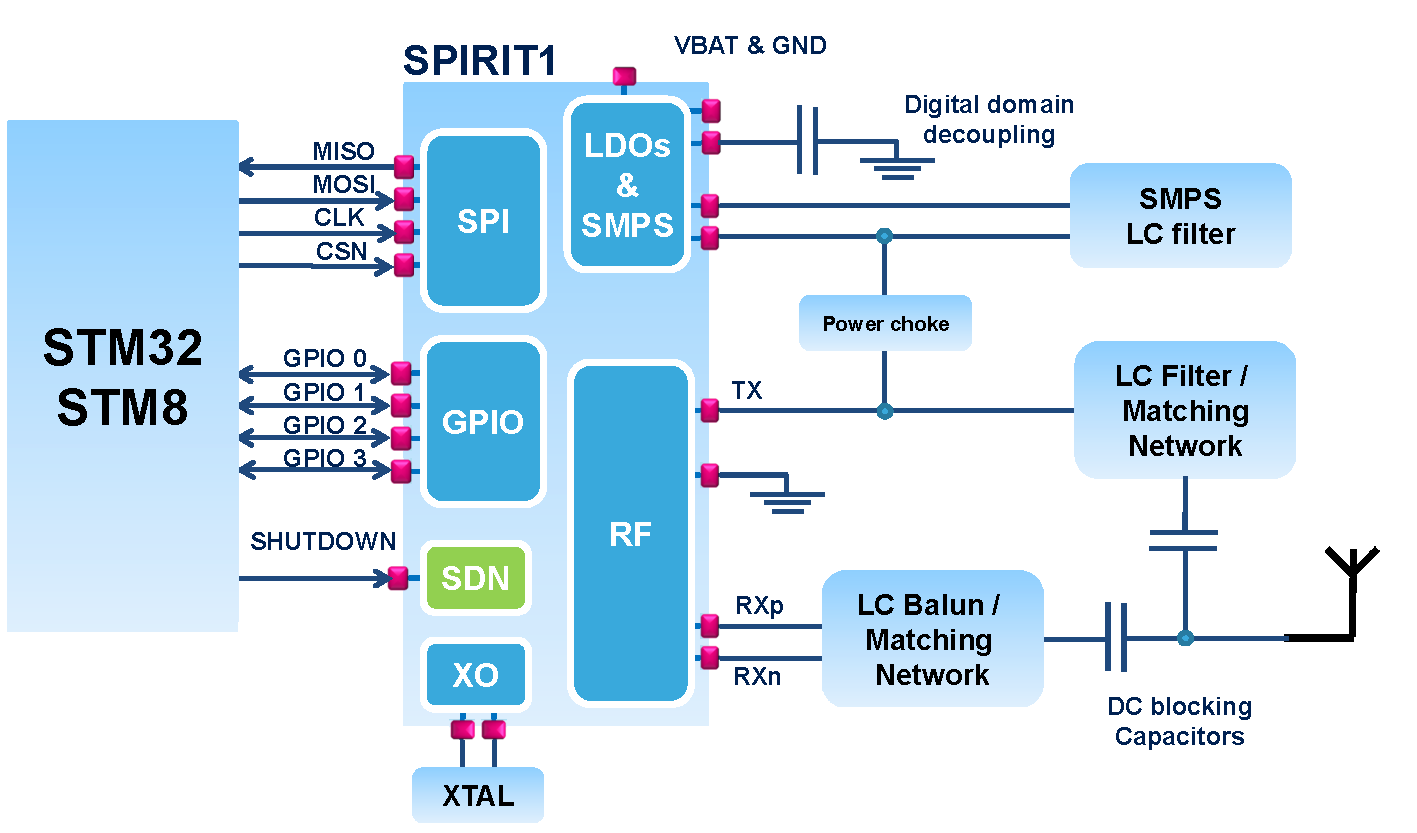
\includegraphics[width=0.8\linewidth]{emcu01.pdf}
      \caption{Aplikační diagram: interface mezi Spirit1 modulem a procesorem}
      \label{EXP001:fig_spirit22}
    \end{figure}   

    \subsection{Provozní režimy a jejich spotřeba}
      \begin{figure}[ht!]  % \ref{EXP001:fig_spirit23}
        \centering
        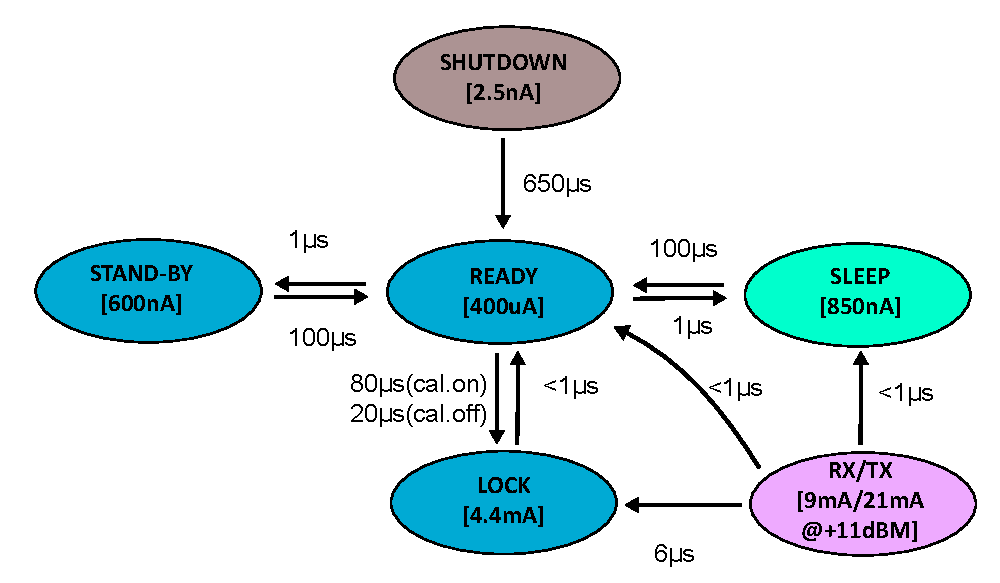
\includegraphics[width=0.8\linewidth]{emcu02.pdf}
        \caption{Provozní režimy: spotřeby a doby přechodů mezi stavy}
        \label{EXP001:fig_spirit23}
      \end{figure}    

      \begin{table}[h]
        \begin{tabular}{lll}
          RX            & 9 mA   & SPI on, XTAL on, Synth on                 \\
          TX            & 21 mA  & SPI on, XTAL on, Synth on                 \\
          Ready         & 400 uA & SPI on, XTAL on                           \\
          Sleep         & 850 nA & SPI on, register retention, RC oscillator \\
          Standby Mode  & 600 nA & SPI on, register retention                \\
          Shutdown Mode & 2.5 nA & Everything OFF                           
          \end{tabular}
      \end{table}


  \section{PA Tx Matching}
    Digitální modulační schémata umožňují využít spínacího principu při konstrukci koncového 
    stupně. Ten totiž není řešen jako konvenční zesilovač třídy A, B, nebo C, ale jako tzv.  
    \emph{switching power amplifier} tj. spínací zesilovač. Tyto zesilovače mají nesrovnatelně 
    vyšší účinnost než konvenční typy, a mají tedy svou funkcí blíže ke spínacím zdrojům, než ke 
    klasickým zesilovačům.   
    
    Následující kapitola pojednává o postupu impedančního přizpůsobení mezi koncovým stupněm se 
    spínaným zesilovačem a anténou: 

    Doporučená literatura:
    \begin{itemize}\addtolength{\itemsep}{-0.5\baselineskip}
      \item Class E – A New Class of High-Efficiency Tuned Single-Ended Switching Power Amplifiers, 
            N. Sokal and Sokal, IEEE Journal of Solid State Circuits, Vol. SC-10, No. 3, June 1975.
      \item Idealized Operation of the Class-E Tuned Power Amplifier, F. Raab, IEEE Transactions on 
            Circuits and Systems, Vol. CAS-24, No. 12, December 1977.
    \end{itemize}
  
    \subsection{Funkce spínacího zesilovače třídy E}       
      Zesilovač je řešen jako spínač, v podobě NMOS tranzistorů v kaskodovém zapojení v open-drain 
      konfiguraci. Obrázek \ref{EXP001:fig_spirit01} ukazuje zapojení typického obvodu impedančního 
      přizpůsobení, nutného pro extrakci vysokofrekvenčního výkonu z výstupu zesilovače.

      Pull-up induktor \(L_{choke}\) je volen tak, aby jeho impedance v okolí pracovního kmitočtu 
      byla co nejvyšší, zatímco obvod (\(L_0 - C_0\)) je volen tak, aby jeho rezonanční 
      kmitočet odpovídal kmitočtu pracovnímu. Kapacitor \(C_{shunt}\) je nutný pro ukládání energie 
      během spínacího cyklu, zároveň je také součástí přizpůsobovacího obvodu tvořeného 
      komponentami \(L_x\) a \(C_x \), které také tvarují výstupní signál v časové  oblasti. Nutno 
      dodat, že toto tvarování je pro spínací zesilovače specifické, a silně ovlivňuje 
      dosaženou účinnost\footnote{Jelikož spínač pracuje v režimu zapnuto - vypnuto, není velikost 
      výstupního výkonu dána amplitudou RF signálu na hradle tranzistoru a nemá tedy smysl definovat 
      zesílení jako poměr výkonů výstupního ku vstupnímu signálu.} samotného zesilovače. 

      \begin{figure}[ht!]  % \ref{EXP001:fig_spirit01}
        \centering
        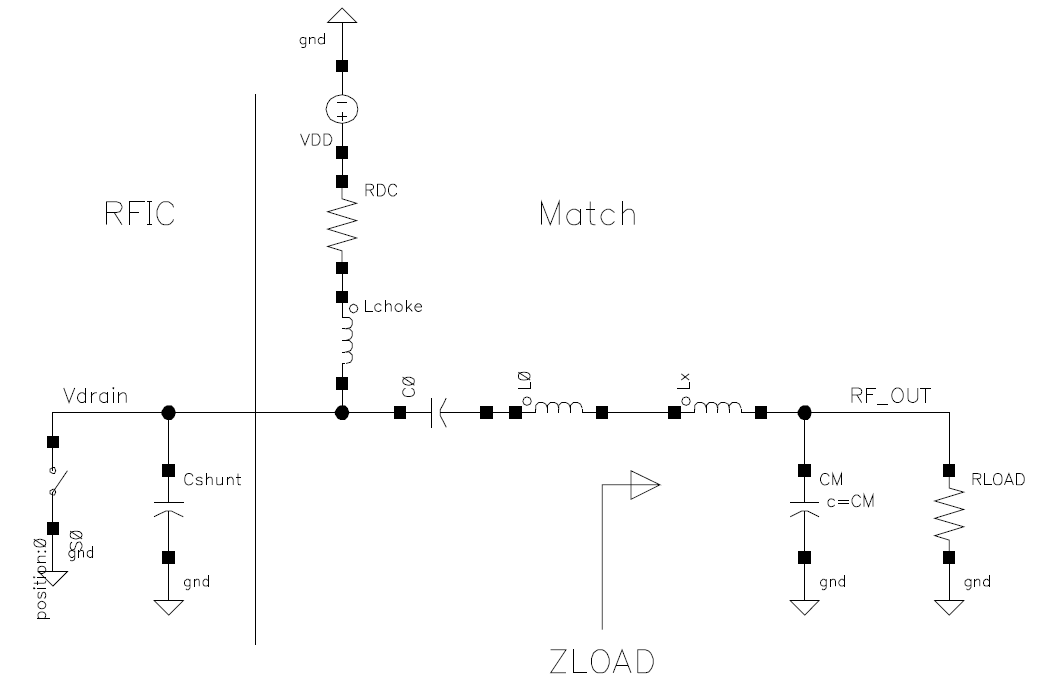
\includegraphics[width=0.8\linewidth]{spirit01_AN732.png}
        \caption{Basic Switching PA Circuit Topology \cite[s.~9]{AN648SiliconLabs}}
        \label{EXP001:fig_spirit01}
      \end{figure}
      
      Velikost výkonu spínacího zesilovače je dána rovnicí \ref{EXP001:eq_spirit01}:
      \begin{equation}\label{EXP001:eq_spirit01}
        P_o = \pi\cdot\omega_0\cdot C_{shunt}\cdot V_{DD}^2
      \end{equation}

      Vztah mezi těmito parametry udává rovnice \ref{EXP001:eq_spirit01}. Všimněme si, že výstupní
      výkon není funkcí impedance zátěže. Je zřejmé, že výkon pro danou pracovní frekvenci lze
      zvětšovat hodnotou kapacity \(C_{shunt}\) (použitelné v integrovaný obvodech), nebo velikostí
      napájecího napětí a to dokonce s kvadrátem.  Čistě teoreticky, třída E dovoluje 100\%
      účinnost\footnote{To je podstatný rozdíl od konvenčních  tříd, kde například třída A má
      teoretickou účinnost 50\% a třída B 78.5\%.}. Je to dáno tím, že ideálním spínačem neteče
      proud v době, kdy je na něm napětí a naopak, viz obrázek  \ref{EXP001:fig_spirit02}.
      
      \begin{figure}[ht!]  % \ref{EXP001:fig_spirit02}
        \centering
        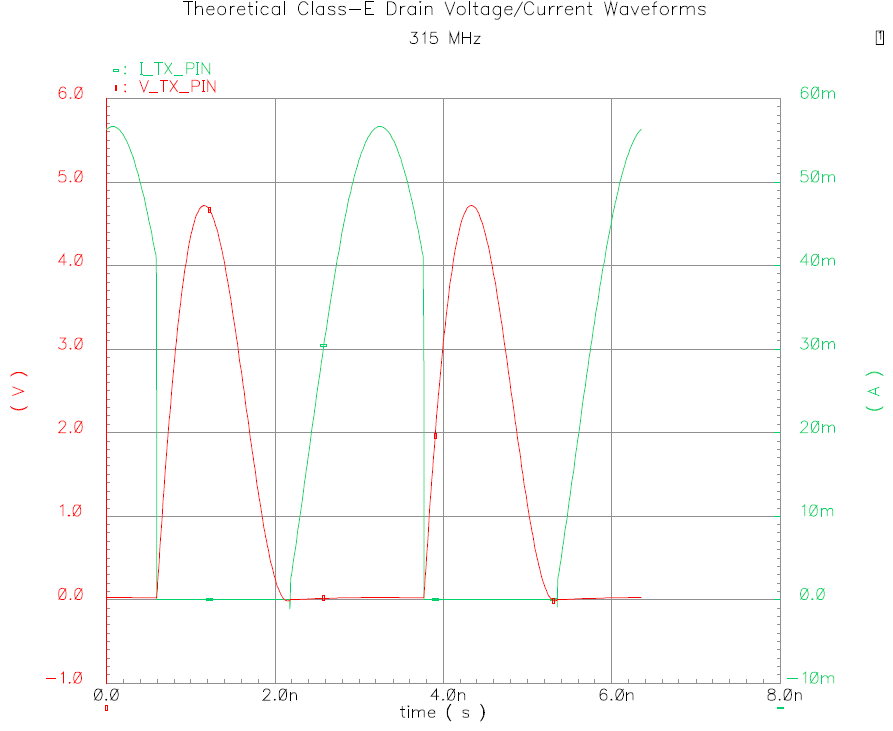
\includegraphics[width=1\linewidth]{spirit02_AN732.png}
        \caption{Teoretické průběhy napětí a proudu zesilovač ve třídě E 
                 \cite[s.~10]{AN648SiliconLabs}}
        \label{EXP001:fig_spirit02}
      \end{figure} 
      
      Prakticky, existují faktory, které dosažení této účinnosti brání: 
      \begin{itemize}\addtolength{\itemsep}{-0.5\baselineskip}
        \item \(V_{DS_{max}}\): špička výstupního napětí dosahuje \(3,56 \times V_{DD}\) 
              % peak of the output voltage waveform in a switching PA may far 
              % exceed this “2xVDD” rule-of-thumb. As is shown in the papers listed above, the 
              % peak drain voltage for a Class-E switching amplifier can reach 3.56 x VDD
        \item \(I_{D_{max}}\), \(R_{DS_{on}} \neq 0\), atd.
      \end{itemize}

    \subsection{Návrhu impedančního přizpůsobení zesilovače třídy E} % Class-E Matching Procedure
      Nejdříve uveďme, souhrný postup a po té provedeme rozbor jednotlivých kroků:
      
      \begin{enumerate}\addtolength{\itemsep}{-0.5\baselineskip}
        \item určit hodnotu \(L_{CHOKE}\) (pull-up induktor), tak aby pro \(f_0\) a pro blízké 
              harmonické měl vysokou impedanci;
        \item stanovit hodnoty \(L_0, C_0\) taky aby vznikl sériový rezonanční článek pro \(f_0\); 
        \item vypočítat hodnotu \(Z_{LOAD}\) na frekvenci \(f_0\). Je nutné do výpočtu zahrunout 
              také hodnotu tzv. \emph{shunt drain capacitance} 
              (\(C_{SHUNT} = \sim\SI{2.5}{\pF}\)\footnote{v katalogovém listu bohužel není uvedena, 
              tato hodnota se uvádí pro Si4438 RFIC od Silicon Labs} okolo frekvence 490 MHz);
        \item stanovit hodnoty \(L_X\) a \(C_M\) pro dosažení přizpůsobení mezi impedancí antény 
              \(R_{ANT} = \SI{50}{\ohm}\)) a vypočítanou hodnotu \(Z_{LOAD}\);
        \item návrh dolní propusti (\emph{Low-pass filter});
        \item provést přizpůsobení vstupu RX - návrh 4-prvkového článku (tzv. balun), který má 
              dvě funkce: impedančně přizpůsobit a konvertovat anténní signál typu single-ended na 
              signál typu differential-ended požadovaný na vstupu přijímače;
      \end{enumerate}
      
      Protože je anténa společná pro příjem a vysílání musíme provést následující korekci:
      \begin{enumerate}\addtolength{\itemsep}{-0.5\baselineskip}
        \item Connect the TX and RX paths together, and deliberately mis-tune L0 by increasing   
              its value if required above its calculated optimum value.
      \end{enumerate}
    
      Class-E Split TX/RX matching procedure; A supply voltage of VDD = 3.3 V and an 
      operation frequency Of 470 MHz is assumed.
      
      \subsubsection{Step 1: Select a Value for LCHOKE Pull-Up Inductor}
        V teoretických výpočtech parametrů zesilovače třídy E, se uvažuje, že impedance  pull-up 
        induktoru \(L_{CHOKE}\) je nulová pro stejnosměrnou složku a nekonečná pro všechny ostatní 
        frekvence. To však není prakticky dosažitelné, a je nutné volit určitý kompromis. Induktory 
        s velkou indukčností mají problém s paralelní vlastní rezonancí selfresonance na požadovaném
        pracovním kmitočtu, proto se bere za dostatečné, když \(L_{CHOKE}\) zajistí vysokou 
        impedanci pouze v okolí \(f_0\).
        
        Přesná hodnota indukčnosti tedy není kritická, avšak doporučují se následující hodnoty: 
        \begin{itemize}\addtolength{\itemsep}{-0.5\baselineskip}
          \item \(\SI{315}{\MHz} : \sim\SI{390}{\nano\henry}\)
          \item \(\SI{470}{\MHz} : \sim\SI{220}{\nano\henry}\)
          \item \(\SI{915}{\MHz} : \sim\SI{100}{\nano\henry}\)
        \end{itemize}
        Těmto hodnotám plně vyhovují induktory o velikosti 0402 nebo 0603.
        
      \subsubsection{Step 2: Choose/Calculate Values for L0-C0 Series-Resonant Tank}
        In Step 2, the L0-C0 tank is designed to be series-resonant at the desired operating 
        frequency Fo. It is self-evident that there are infinite combinations of L0-C0 values that 
        can achieve resonance at a desired frequency. However, certain broad guidelines may be used 
        to select one particular solution of component values.
        
        First, the inductance and capacitance values should be neither extremely large or extremely 
        small. Discrete inductors and capacitors with extremely large values are subject to 
        degrading effects due to self-resonance. Discrete components with extremely small values 
        are also subject to degrading effects due to component tolerance. In either case, the 
        actual resonant frequency of the tank may be significantly different than the frequency 
        predicted by mathematical calculations. Second, in the theoretical derivation for Class-E 
        switching amplifiers it is desired that the impedance of the L0-C0 series-resonant tank be 
        zero at Fo and infinite at all other frequencies. This is not achievable in practice; 
        however, a reasonable approximation to this performance may be obtained by using values 
        with a high L-to-C ratio.
        
        Third, it is desirable to minimize the insertion loss of the resonant tank. As the quality 
        factor (Q) of discrete inductors is generally much lower than that of discrete capacitors, 
        it is important to select an L0-C0 ratio that maximizes the inductor Q. The Q of discrete 
        inductors generally increases as the inductance value is also increased, until the 
        inductance approaches the value where self-resonance becomes a concern.
        
        Finally, it is desirable to select component values that are near standard 5\% tolerance 
        values. These considerations lead to the following guidelines for selecting the values for 
        L0-C0:
        \begin{itemize}\addtolength{\itemsep}{-0.5\baselineskip}
          \item The L0-C0 tank must resonate at Fo
          \item The value of L0 should be chosen as large as possible,
          \item While remaining low enough that effects of self-resonance are not an issue,
          \item And are close to standard 5\% tolerance values
        \end{itemize}
        
        Assuming a desired operating frequency of Fo = 470 MHz as an example, these guidelines lead 
        to selection and/or calculation of the following values for L0-C0:
        \begin{itemize}\addtolength{\itemsep}{-0.5\baselineskip}
          \item C0 = 8.2 pF (chosen)
          \item L0 = 13.903 nH (calculated)
        \end{itemize}
        
      \subsubsection{Step 3: Calculate the Required Value for ZLOAD}
        In Step 3, the required value of load impedance is calculated. This represents the 
        impedance that must be presented to the output of the L0-C0 resonant tank, and is 
        calculated at the fundamental operating frequency Fo.
        
        In the theoretical derivation for Class-E switching amplifiers, it is shown that the 
        required load impedance (ZLOAD) is a function of shunt drain capacitance (CSHUNT) and 
        operating frequency \(\omega_o = 2\pi f_o\) as follows:
        \begin{equation}\label{EXP001:eq_spirit02}
          Z_{LOAD_{fund}} = \left(\frac{0.2815}{\omega_oC_{shunt}}\right)e^{j49.0524°}
        \end{equation}
        
        This equation states that the required load impedance (ZLOAD) does not vary with the 
        desired level of output power, but depends only on the desired operating frequency and 
        value of shunt drain capacitance. The value of internal shunt drain capacitance CSHUNT is a 
        design parameter of the Si4438 RFIC and is not adjustable by the user. This shunt 
        capacitance is composed primarily of the drain-source capacitance (Cds) of the output MOS 
        devices. Silicon Laboratories states that the value of this internal shunt drain 
        capacitance is approximately:          
        \begin{equation}\label{EXP001:eq_spirit03}
          C_{SHUNT} \sim \SI{2.5}{pF}
        \end{equation}          
        
        Assuming a desired operating frequency of Fo = 470 MHz as an example, the following value 
        for ZLOAD may be calculated:
        \begin{equation}\label{EXP001:eq_spirit04}
          Z_{LOAD(470\,MHz)} = 
            \left(\frac{0.2815}{2\pi\cdot\SI{470}{MHz}\cdot\SI{2.5}{pF}}\right)e^{j49.0524°} =
            24.87 + j28.66\Omega
        \end{equation} 
        
        This value of load impedance (ZLOAD) is not the same parameter as the antenna impedance 
        (ZANT), nor do they necessarily have the same ohmic value. A matching network must be 
        constructed that transforms the arbitrary value of antenna impedance ZANT into the required 
        value of load impedance ZLOAD, as seen at the output of the L0-C0 resonant circuit.
        \begin{equation}\label{EXP001:eq_spirit05}
          V_{DD_{PA}} = \sqrt{\frac{P_{out}}{\pi\omega_oC_{shunt}}}
        \end{equation}
        Continuing the design example of 470 MHz and assuming a desired output power of +20 dBm 
        (100 mW), the required value of VDD\_PA may be calculated:
        \begin{equation}\label{EXP001:eq_spirit06}
          V_{DD_{PA}} =\sqrt{\frac{\SI{0.1}{W}}{2\pi^2\SI{470}{MHz}\cdot\SI{2.5}{pF}}} = \SI{2.076}{V}
        \end{equation}
        This equation states that if the voltage supplied to the top of pull-up inductor LCHOKE is 
        equal to 2.076 V and the previously-calculated value of load impedance ZLOAD is presented 
        to the chip, the resulting output power will be POUT = 100 mW = +20 dBm.
        
        This required PA supply voltage (VDD\_PA) is significantly different than the general 
        supply voltage (VDD) for the rest of the RFIC. It is obviously not desirable to maintain 
        two separate, independent sources of supply voltage for the RFIC; therefore, it is 
        convenient to create the PA output supply voltage from the main supply voltage by means of 
        an I-R voltage drop across a resistor or a properly adjusted internal switcher loss.
        
        As the theoretical efficiency of a Class-E switching amplifier is 100\%, the average PA 
        drain current IDD\_PA may be calculated as:
        \begin{equation}\label{EXP001:eq_spirit07}
          P_{OUT} = \pi\omega_0C_{SHUNT}V_{DD_{PA}}^2 = I_{DD_{PA}} \cdot V_{DD_{PA}}
        \end{equation}
        This equation may be solved for \(I_{DD_{PA}}\) to obtain:
        \begin{equation}\label{EXP001:eq_spirit08}
          I_{DD_{PA}} = \pi\omega_0C_{SHUNT}V_{DD_{PA}}^2 = I_{DD_{PA}} \cdot V_{DD_{PA}}
        \end{equation}
        Given the main supply voltage for the remainder of the chip (VDD), and having previously 
        calculated the required value of PA supply voltage (VDD\_PA) and average PA drain current 
        (IDD\_PA), it is a simple matter to calculate the required value for RDC:
        \begin{equation}\label{EXP001:eq_spirit09}
          R_{DC} = \frac{V_{DD} - V_{DD_{PA}}}{I_{DD_{PA}}}
        \end{equation} 
        Continuing the design example of 470 MHz for +20 dBm output power, the following 
        calculations are made:
        \begin{equation}\label{EXP001:eq_spirit10}
          I_{DD_{PA}} = 2\pi^2\cdot\SI{470}{MHz}\cdot\SI{2.5}{pF}\cdot\SI{2.076}{V} = \SI{48.16}{mA}
        \end{equation} 
        Assuming a general chip supply voltage of VDD = 3.3 V, the required value of RDC may be 
        calculated as:
        \begin{equation}\label{EXP001:eq_spirit11}
          R_{DC} = \frac{\SI{3.3}{V} - \SI{2.076}{V}}{\SI{48.16}{mA}}  = \SI{25.41}{\ohm}
        \end{equation} 
        
        Theoretically, this value of resistance must be placed in series with LCHOKE in order to 
        drop the general chip supply voltage down to the value required to obtain the desired 
        output power.
        
        However, these calculations for the value of RDC assume theoretically-ideal Class-E 
        operation. In practice, the circuit will not behave exactly as predicted by these equations 
        due to non-idealities such as non-zero ON-state resistance, finite OFF-state resistance, 
        non-zero switching times, and loss in the external matching components. As a result, the 
        output power obtained for a given value of VDD supply voltage will almost certainly be 
        slightly less than predicted by theory. Stated another way, it will almost always be 
        necessary to use a smaller value of RDC than predicted by theory in order to obtain the 
        desired value of output power. Some amount of post-calculation “tweaking” of the component 
        values is considered a normal part of the PA matching process, especially if the tuning of 
        the switcher’s ON-state resistance is used instead of an external RDC. In this case, a 
        tweaking of the power state is required at the applied supply voltage.
      
      \subsubsection{Step 5: Calculate the Values for Matching Components LX and CM}
        In Step 5, the values of the matching components (LX and CM) required to transform the 
        given antenna impedance (ZANT) into the required load impedance (ZLOAD) are calculated.
        
        This matching effort may be accomplished by simple and normal design methods, such as use 
        of a Smith Chart or impedance matching CAD software (e.g., WinSmith™). Continuing the 
        design example for 470 MHz and assuming an antenna impedance of ZANT = RANT = 50 Ω, it is 
        found that a shunt capacitance CM = 6.81 pF and series inductance LX = 18.17 nH is required 
        to transform RANT = 50 Ω to the required value of ZLOAD = 24.87 + j 28.66 Ω. The resulting 
        circuit topology is shown in 
        figure \ref{EXP001:fig_spirit01}.
        
        This is only one possible solution for the required impedance transformation; other 
        matching topologies could have been used as well. The reader should also note that the 
        required LX-CM match topology depends upon the real part of the load impedance, Re(ZLOAD). 
        In this example, the real part of the load impedance was less than 50 Ω and thus an 
        appropriate matching topology consisted of a shunt capacitor (CM) and a series inductor 
        (LX). In the event that Re(ZLOAD) had been greater than 50 Ω, an appropriate matching 
        topology would have consisted of first a series inductor (LX) followed by a shunt capacitor 
        (CM).
        
        It is apparent that series inductors L0 and LX may be combined into one equivalent inductor 
        with a value equal to the sum of their individual inductances, in order to reduce parts 
        count. This is a normal and usual practice.
        
        In the example shown here, the following component values (obtained through use of the 
        above design equations) were obtained:
        
        \begin{itemize}\addtolength{\itemsep}{-0.5\baselineskip}
          \item Fo = 470 MHz
          \item POUT(TARGET) = +20 dBm
          \item VDD = 3.3 V
          \item CSHUNT = 2.5 pF
          \item LCHOKE = 220 nH
          \item RDC = 25.41 Ω
          \item C0 = 6.81 pF
          \item L0+LX = 32.15 nH
          \item CM = 6.81 pF          
        \end{itemize}
        
        In practice, these exact values would be rounded to the nearest available 5\% tolerance 
        parts (e.g., L0+LX = 30 nH, CM = 6.8 pF, RDC=24 ohms). Also, as mentioned previously, the 
        external RDC resistor is not used in the Si4428 matching. Instead the internal switcher 
        on-state resistance is adjusted properly by the power setting (PDAC register value).
        
      \subsubsection{Step 6: Design a Lowpass Filter}
        In Step 6, a low-pass filter network is designed in order to attenuate the harmonics below 
        the level required to meet applicable regulatory standards (e.g., FCC or ETSI).
        
        The signal at the output of the match shown in Figure 5 will likely contain relatively high 
        levels of harmonics. Although the bandpass response of the series-resonant L0-C0 tank 
        provides some attenuation of harmonic signals, it is generally not sufficient to meet 
        applicable regulatory standards. This is normal for such a switching-amplifier and matching 
        topology.
        
        It is difficult for Silicon Laboratories to recommend one single low-pass filter design 
        that is appropriate for all customers, as customers may operate under widely differing 
        regulatory standards and harmonic requirements. Also, the radiation efficiency of the 
        antenna selected by the customer is not known in advance. These factors make it difficult 
        for Silicon Laboratories to conclusively state the required filter attenuation 
        characteristics. As a reasonable compromise, the following 
        design goals for the low-pass filter are chosen:
        \begin{itemize}\addtolength{\itemsep}{-0.5\baselineskip}
          \item Minimal insertion loss at the desired operating frequency
          \item Lowest filter order possible to achieve harmonic attenuation required to meet 
                regulatory standard
          \item impedance transformation (i.e. \SI{50}{\ohm} input and \SI{50}{\ohm} output 
                impedance)          
        \end{itemize}
        
        Note that the amplitude characteristics of the LPF in the lower portion of the passband are 
        relatively unimportant. Because the output signal contains no frequency components below 
        the fundamental frequency, the frequency response of the filter below the desired operating 
        frequency is of little consequence. It is therefore acceptable to select the filter type 
        (e.g., Butterworth, Chebyshev, Elliptic) based primarily upon the filter’s attenuation 
        characteristics rather than its passband response.
        
        A Butterworth filter design is sub-optimal because it provides relatively poor 
        high-frequency attenuation characteristics; there is no need to sacrifice high-frequency 
        attenuation in order to obtain a maximally-flat in-band frequency response.
        
        Similarly, an Elliptic filter design (Cauer-Chebyshev) may provide insufficient attenuation 
        at higher-order harmonic frequencies. While it may be possible (and advantageous) to tune a 
        transmission zero in the stopband to the exact frequency of a problematic harmonic (e.g., 
        N=2 or N=3), it is paid for with a decrease in attenuation at higher harmonic frequencies. 
        Insufficient attenuation of higher-order harmonics may result.
        
        As a result, a Chebyshev low-pass filter design is settled upon as an acceptable type of 
        filter response. With a Chebyshev filter, it is possible to obtain a greater rate of 
        attenuation roll-off in the stopband by accepting a larger amount of amplitude ripple in 
        the passband. However, this design trade-off should not be pushed too far. By designing for 
        a limited amount of passband amplitude ripple, an upper limit is placed on the filter 
        insertion loss due to mistuning of the component values and thus accidentally operating on 
        a minimum of the amplitude ripple response rather than on a maximum. Silicon Laboratories 
        recommends a Chebyshev passband amplitude ripple of 0.25 dB to 0.5 dB as providing a 
        reasonable balance between high-frequency stopband attenuation and potential passband 
        filter insertion loss due to component tolerance.
       
        \begin{figure}[ht!]  % \ref{EXP001:fig_spirit03}
          \centering
          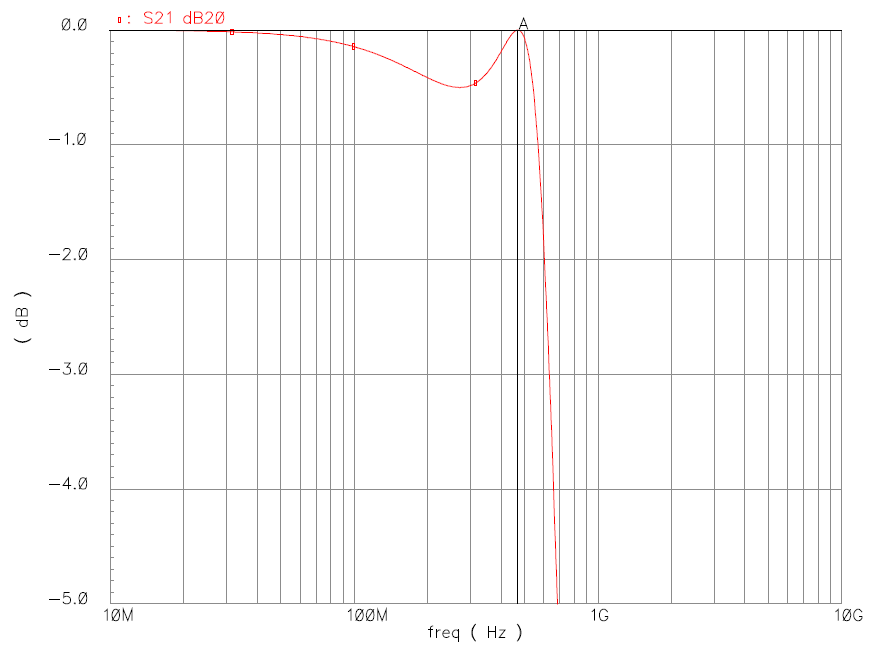
\includegraphics[width=1\linewidth]{spirit03_AN732.png}
          \caption{Ideal \(3^{rd}\)-Order 0.5 dB Chebyshev Filter Response at 470 MHz 
                   \cite[s.~18]{AN648SiliconLabs}}
          \label{EXP001:fig_spirit03}
        \end{figure} 
        
        Figure \ref{EXP001:fig_spirit03} shows the passband frequency response of an ideal 
        (lossless) Chebyshev filter with 0.5 dB of amplitude ripple in the passband. In order to 
        minimize the insertion loss of the filter at the desired operating frequency, it is 
        necessary to design the cutoff frequency of the filter such that the desired operating 
        frequency falls at one of the  passband amplitude ripple peaks (Cursor “A” in the plot). If 
        the desired operating frequency fell on a minimum of the amplitude ripple response (rather 
        than on a maximum), the filter insertion loss would increase and the TX output power would 
        decrease.
        
        Filter component values may be obtained by usual design methods, such as use of Filter 
        Design CAD software or tables of normalized filter values scaled to the desired frequency 
        of operation. Note that Silicon Laboratories recommends designing the filter such that the 
        desired operating frequency falls at a peak of the amplitude ripple response rather than at 
        the 3 dB cutoff frequency or at the equal amplitude ripple cutoff frequency. In this 
        manner, the insertion loss of the filter will be minimized, and the TX output power will be 
        maximized. For a 3rd-order 0.1 dB
        
        Chebyshev filter, the ratio of F3dB:FPEAK is approximately 1.60:1. That is, if the desired 
        operating frequency is 470 MHz, the filter must be designed for a 3 dB cutoff frequency of 
        470 x 1.60 = 752 MHz. For a 3rd-order 0.5 dB
        
        Chebyshev filter, the ratio of F3dB:FPEAK is approximately 1.346:1. SPICE model simulations 
        of non-ideal discrete components predict an in-band filter insertion loss of approximately 
        1.0 dB at the desired operating frequency (470 MHz, in this example). While not desirable, 
        this value of filter insertion loss is fairly realistic, given the typical Qs of discrete 
        components in 0402-size or 0603-size surfacemount packages. Discrete components of higher 
        quality (e.g. wire-wound inductors) may be chosen in an effort to reduce insertion loss, 
        but such parts are admittedly more expensive. The Si4438 RFIC is capable of providing the 
        specified output power (+20 dBm) at the antenna output connector (i.e., after the insertion 
        loss of the match and lowpass filter)
        
      \subsubsection{Step 7: Design RX Input Match}
        The mathematical derivation for the required component values has been thoroughly described 
        in “AN643: Si446x RX LNA Matching”; the relevant equations from that document are shown 
        here.
   
  \section{RX LNA Matching}
    The LNA on the Spirit1 is designed as a differential amplifier and thus has two input pins (RXp 
    and RXn) on the RFIC. It is necessary to design a network that not only provides a conjugate 
    match to the input impedance of the LNA but also provides a balanced-to-unbalanced conversion 
    function (i.e., a balun).
    
    The LNA design is differential and thus the RXp and the RXn input pins may be considered 
    interchangeable. Although the figures in this document may show the matching components 
    connected to the RXp/RXn pins in a certain fashion, the pin connections may be reversed without 
    change in functionality.
    
    Use of two basic matching network topologies will be considered within this application note.
    \begin{itemize}\addtolength{\itemsep}{-0.5\baselineskip}
      \item Three-Element Match Network
      \item Four-Element Match Network
    \end{itemize}
    
    \subsection{Three-Element Match Network}
      The simplest match network that may be fabricated from discrete components is comprised of 
      three discrete elements. Two forms of the 3-element match network may be constructed: one 
      with a highpass filter (HPF) response, and one with a lowpass filter (LPF) response. However, 
      the form with a lowpass filter response is not realizable at all frequencies and input 
      impedances. As a result, only the form with a highpass filter response is discussed within 
      this document.
      
      A 3-element (CR1-LR1-CR2) HPF matching network is shown in Figure \ref{EXP001:fig_spirit07}. 
      This matching network has the virtue of requiring a minimum number of components but results 
      in slightly sub-optimal performance. It is not theoretically possible to achieve a perfectly 
      balanced single-ended-to-differential conversion function with this matching network for 
      input impedances with finite values of RLNA. As will be demonstrated, the waveforms obtained 
      at the RXp and RXn inputs to the RFIC will not be exactly 180° out of phase; the result is a 
      very slight loss in conversion gain in the LNA and a small drop in overall sensitivity of the 
      RFIC. The reduction in performance is typically less than 0.5 dB; many customers may view 
      this as an acceptable trade-off for the reduction in the bill of materials (BOM).
      
      The RXp and RXn inputs of the Si446x/Si4362 RX LNA internally contain high value 
      (~\SI{15}{k\ohm}) pull-down resistors to GND. As a result, supplying a dc voltage to these 
      pins is not recommended; use of external ac-coupling to these pins is suggested. This is 
      inherently supplied by capacitor CR2 of Figure \ref{EXP001:fig_spirit07}.

      \begin{figure}[ht!]  % \ref{EXP001:fig_spirit07}
        \centering
        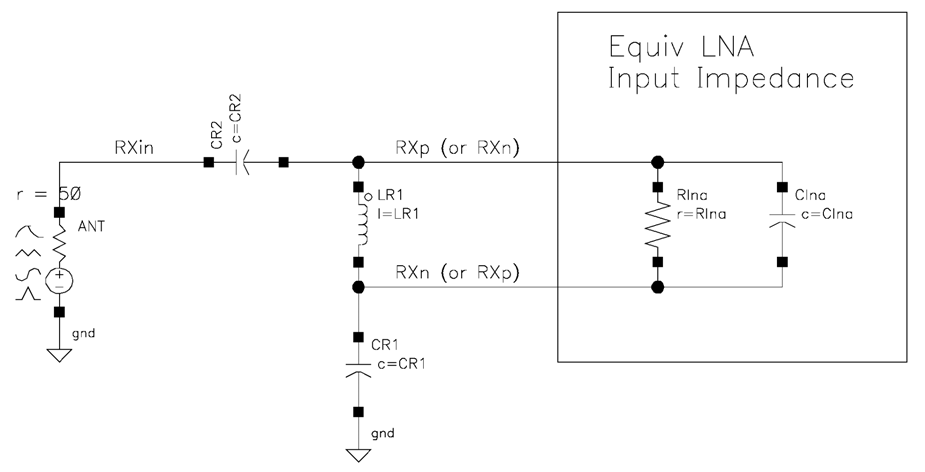
\includegraphics[width=1\linewidth]{spirit07_AN732.png}
        \caption{HPF Three-Element Match Network \cite[s.~2]{AN643SiliconLabs}}
        \label{EXP001:fig_spirit07}
      \end{figure}
      
    \subsection{Four-Element Match Network}
      For those customers concerned with obtaining optimal performance, the 4-element match network 
      of Figure \ref{EXP001:fig_spirit08} is recommended. This match network can provide 
      theoretically perfect phase balance between the RXp and RXn inputs (exactly 180° 
      out-of-phase), thus optimizing LNA conversion gain and receiver sensitivity. The only 
      drawback is the addition of one more component (an inductor) to the BOM. Use of this matching 
      topology is also mandatory for circuit configurations in which the TX and RX paths are tied 
      directly together without use of an RF switch. This is discussed in greater detail in 
      "4.2.8. Use of 4-Element Match Network in Direct Tie Board Configurations" on page 22.
      \begin{figure}[ht!]  % \ref{EXP001:fig_spirit08}
        \centering
        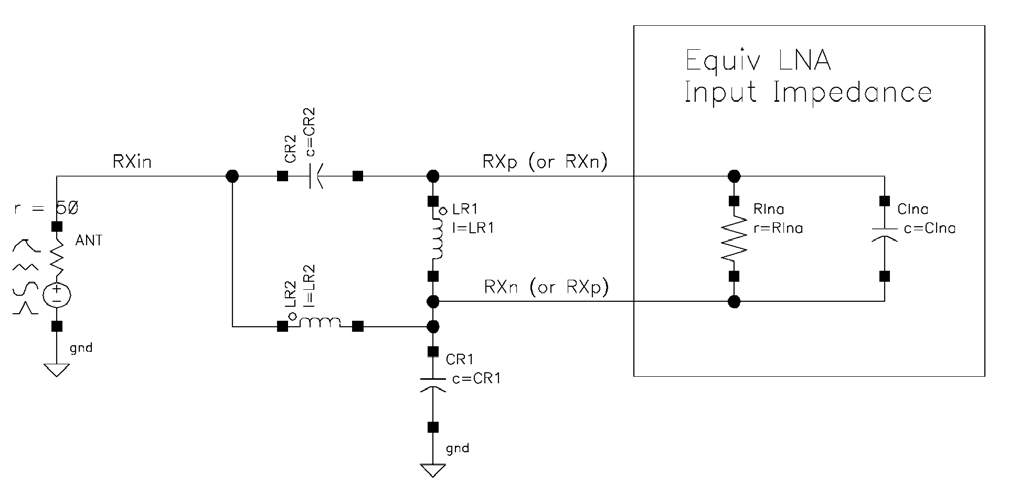
\includegraphics[width=1\linewidth]{spirit08_AN732.png}
        \caption{Four-Element Match Network \cite[s.~3]{AN643SiliconLabs}}
        \label{EXP001:fig_spirit08}
      \end{figure}
    
    \subsection{Differential LNA Input Impedance} 
      Silicon Laboratories has measured the differential input impedance of the Si4461 RX LNA 
      directly at the RXp/RXn input pins of the RFIC, with no matching network. Although this 
      measurement was taken on a Si4461 chip, the data is applicable to other members of the Si446x 
      family of chips and also on the Si4362, as the LNA is similar in all devices.
      
      The plot shown in Figure \ref{EXP001:fig_spirit09} shows the measured differential input 
      impedance in the RX mode of operation over the 140 to 960 MHz frequency band, with markers 
      placed at various points throughout the frequency range.
      
      \begin{figure}[ht!]  % \ref{EXP001:fig_spirit09}
        \centering
        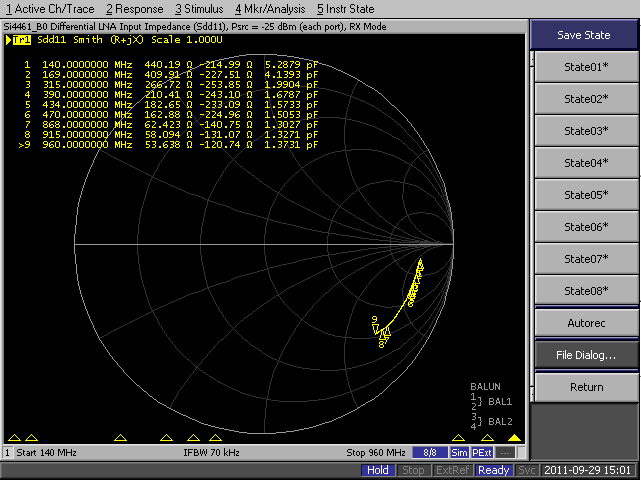
\includegraphics[width=1\linewidth]{spirit09_AN732.png}
        \caption{Si446x/Si4362 Differential RX LNA Input Impedance 140-960 MHz (RX Mode) 
                 \cite[s.~4]{AN643SiliconLabs}}
        \label{EXP001:fig_spirit09}
      \end{figure}
       
      As can be seen from this curve, at any given single frequency the input impedance of the LNA 
      may be considered as a resistance in parallel with a small amount of capacitance. That is to 
      say, the input impedance of the LNA falls in the capacitive half of the Smith Chart across 
      its entire operating frequency range.
      
      The impedance curve shown in Figure \ref{EXP001:fig_spirit09} cannot be described by a single 
      fixed value of resistance, placed in parallel with a single fixed value of capacitance. The 
      equivalent values of  parallel resistance and capacitance (RLNA and CLNA in Figure 1 and 
      Figure 2) vary as a function of frequency. However, the variation with frequency is not 
      rapid; it is possible to construct a moderately wideband (~100 MHz) matching network by 
      simply designing for the value of RLNA and CLNA in the center of the desired frequency range.
      
      From the differential input impedance values (Z = R + jX) shown in Figure 9, it is necessary 
      to first calculate the equivalent input admittance, where Y = 1/Z = G + jB. It is then a 
      simple matter to calculate the values of the equivalent input resistor and capacitor (i.e., 
      RLNA and CLNA in Table 1) as RLNA = 1/G and CLNA = B/(2πFRF).
     
    \subsection{Three-Element Matching Procedure}
      \subsubsection{Step 1: Plot the LNA Input Impedance}
        The matching procedure begins with the equivalent parallel RLNA-CLNA circuit values 
        obtained from Table 1. At 470 MHz, the equivalent circuit values are found to be RLNA = 474 
        Ω and CLNA = 0.99 pF. It is useful to plot this value on a Smith Chart, as shown in Figure 
        \ref{EXP001:fig_spirit10}
        \begin{figure}[ht!]  % \ref{EXP001:fig_spirit10}
          \centering
          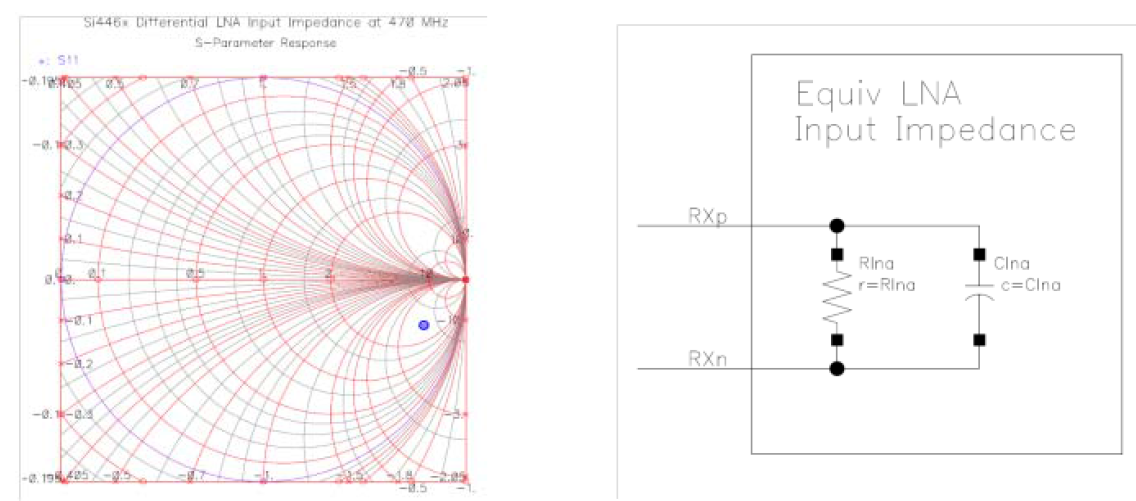
\includegraphics[width=1\linewidth]{spirit10_AN732.png}
          \caption{Step 1: Plot LNA Input Impedance \cite[s.~6]{AN643SiliconLabs}}
          \label{EXP001:fig_spirit10}
        \end{figure}
        
      \subsubsection{Step 2: Add Parallel Inductance LLNA to Resonate with LNA Capacitance}
        Although Step 2 may technically be combined with the subsequent Step 3, the design 
        equations are somewhat easier to manipulate if the equivalent LNA input capacitance CLNA is 
        first effectively cancelled (at the frequency of interest) by resonating it with a parallel 
        inductance LLNA.
        \begin{equation}\label{EXP001:eq_spirit12}
          L_{LNA} = \left(\frac{1}{\omega_0^2\cdot C_{LNA}}\right)
        \end{equation}
        
        In the design example at 470 MHz, this value of inductance is calculated to be equal to 
        LLNA = 115.83 nH. After this amount of parallel inductance is added across the LNA inputs, 
        the input impedance can be considered to be purely real and of a value equivalent to RLNA. 
        This is shown in Figure 
        \ref{EXP001:fig_spirit11}.
        
        \begin{figure}[ht!]  % \ref{EXP001:fig_spirit11}
          \centering
          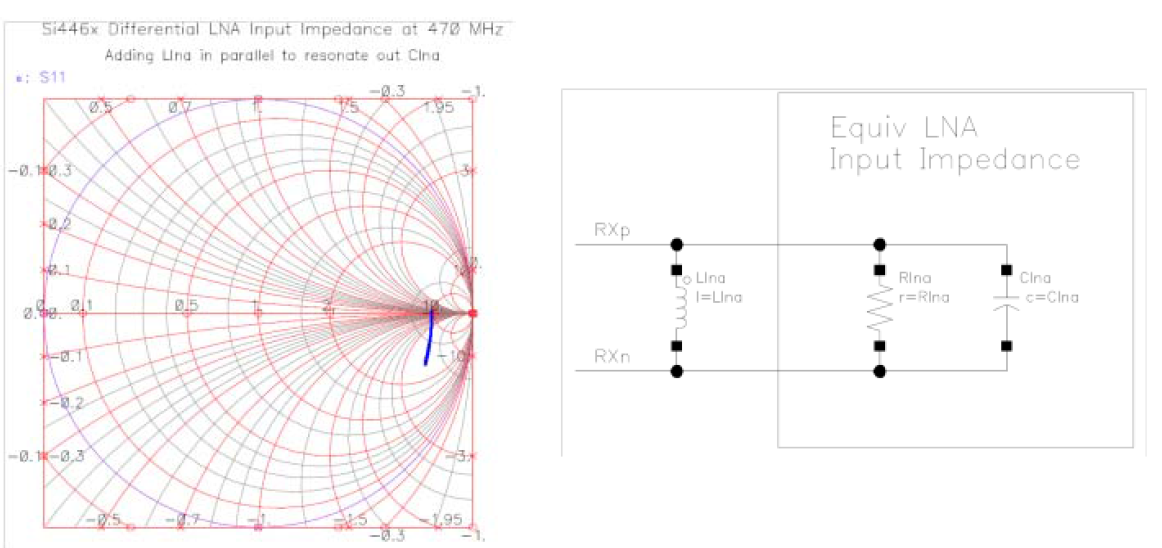
\includegraphics[width=1\linewidth]{spirit11_AN732.png}
          \caption{Step 2: Add Parallel Inductance to Resonate CLNA \cite[s.~7]{AN643SiliconLabs}}
          \label{EXP001:fig_spirit11}
        \end{figure}
        
      \subsubsection{Step 3: Place Additional Matching Inductance in Parallel with LNA Input}
        Next an additional matching inductor LM is placed in parallel with the LNA input network. 
        The value of the inductance should be chosen to further rotate the susceptance on the Smith 
        Chart along a line of constant conductance (in the -jBP direction) until the 50 Ω circle is 
        reached (assuming the antenna source impedance is 50 Ω). The required value of matching 
        inductance LM is given by the following:
        
        \begin{equation}\label{EXP001:eq_spirit13}
          L_M = \frac{1}{\omega_0\cdot\sqrt{\left(\dfrac{1}{\SI{50}{\ohm}\cdot R_{LNA}}\right) - 
                         \left(\dfrac{1}{R_{LNA}}\right)^2}}
        \end{equation}
        
        Using this equation, or by employing graphical methods on the Smith Chart, the additional 
        parallel matching inductance required to reach the 50 Ω circle is found to be LM = 55.12 nH.

        \begin{figure}[ht!] %\ref{EXP001:fig_spirit12}
          \centering
          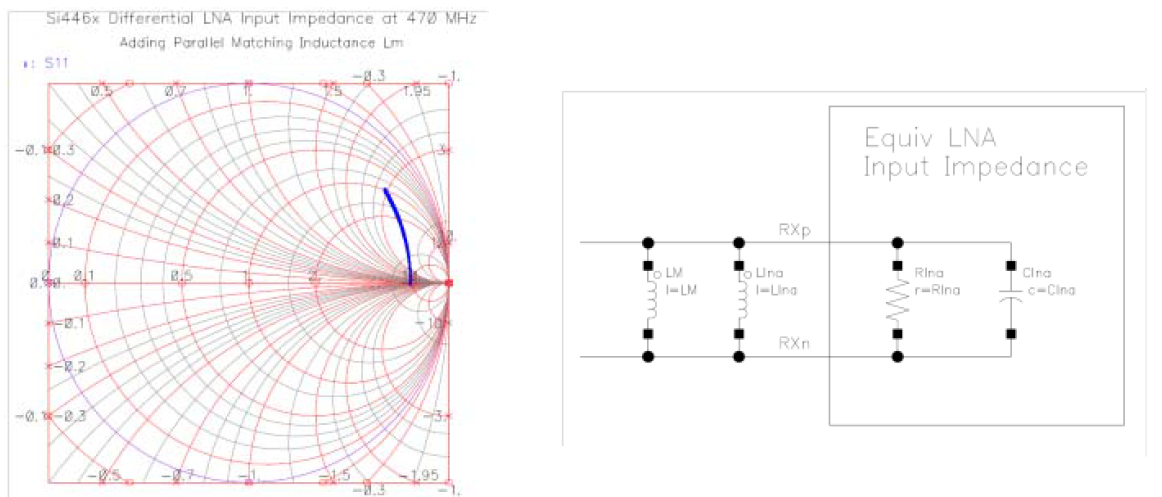
\includegraphics[width=1\linewidth]{spirit12_AN732.png}
          \caption{Step 3: Add Parallel Matching Inductance LM \cite[s.~7]{AN643SiliconLabs}}
          \label{EXP001:fig_spirit12}
        \end{figure}
        
        As LLNA and LM are in parallel with each other, they may be combined into one equivalent 
        inductance LR1.
        \begin{equation}\label{EXP001:eq_spirit14}
          L_{R1} = \frac{L_{LNA}\cdot L_M}{L_{LNA} + L_M}
        \end{equation}
        Using this equation, it is quickly determined that a single inductor of value LR1 = 37.35 
        nH may be used in place of LLNA and LM.
        
      \subsubsection{Step 4: Determine Total Amount of Series Capacitive Reactance}
        It is next necessary to determine the total amount of series capacitive reactance 
        (-jXCTOTAL) required to match this point to 50 Ω. That is to say, it is desired to rotate 
        the reactance along a line of constant resistance until arriving at the center of the Smith 
        Chart. The required value of total capacitance is given by the following:
        \begin{equation}\label{EXP001:eq_spirit15}
          C_{TOTAL} = \frac{1}{\omega_0\cdot\SI{50}{\ohm}\sqrt{\dfrac{R_{LNA}}{\SI{50}{\ohm}}-1}}
        \end{equation}
        Using this equation, or by employing graphical methods on the Smith Chart, the total series 
        capacitance required to reach the 50 Ω origin of the Smith Chart is found to be CTOTAL = 2.33 pF.
        
        \begin{figure}[ht!] %\ref{EXP001:fig_spirit13}
          \centering
          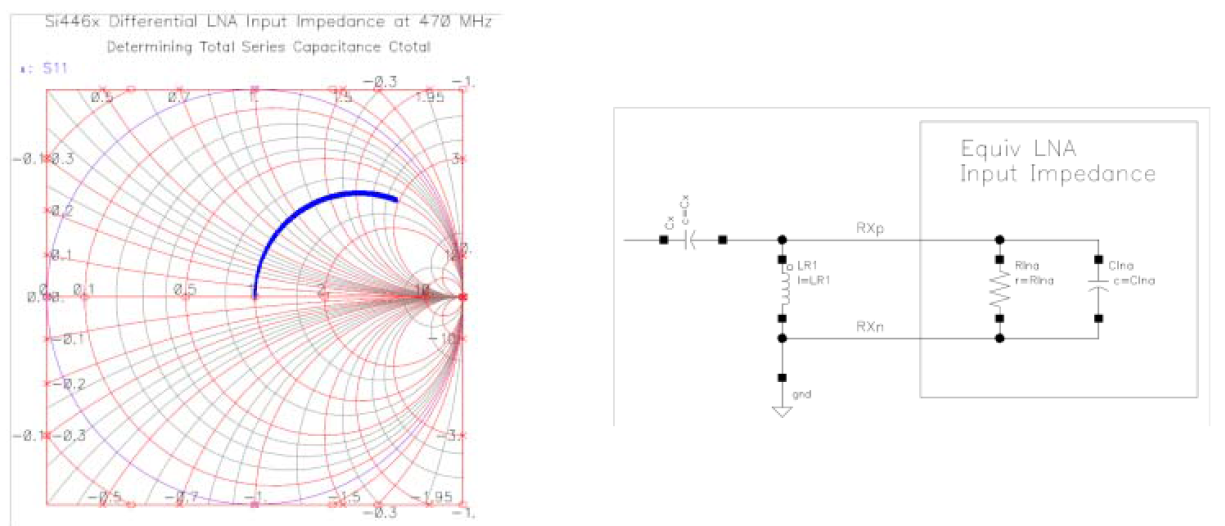
\includegraphics[width=1\linewidth]{spirit13_AN732.png}
          \caption{Step 4: Determine TOTAL Series Capacitive Reactance \cite[s.~8]{AN643SiliconLabs}}
          \label{EXP001:fig_spirit13}
        \end{figure}
        
      \subsubsection{Step 5: Allocate Total Series Capacitance between CR1 and CR2}
        The final step is to properly allocate this total required series capacitive reactance 
        between CR1 and CR2. There are an infinite number of possible matching networks which 
        achieve a perfect match to 50 Ω. However, only one of these solutions also achieves the 
        best possible equal amplitude with 180°phase relationship between the waveforms at the RXp 
        / RXn inputs.
        
        For example, it would be possible to set the value of CR1 so large that it provides 
        essentially 0 Ω of capacitive reactance and essentially ac-shorts the RXn pin to GND. Under 
        this condition, it would be possible to set the value of CR2 to provide all of the required 
        series capacitive reactance (determined in Step 4 above) and still achieve a perfect match 
        to 50 Ω. However, it is clear that the waveforms at the RXp and RXn nodes would not be 
        balanced. The voltage at the RXn pin in this scenario would be zero (ac-shorted to GND by 
        CR1). From an ac standpoint, this is equivalent to the schematic shown in Figure 
        \ref{EXP001:fig_spirit13}
        
        To properly allocate the total series capacitive reactance between CR1 and CR2, the 
        required relationship between LR1 and CR1 must first be recognized. It is desirable for the 
        voltages at the RXp and RXn pins to be equal in amplitude but opposite in phase, and thus 
        the voltage developed “across” the parallel network of LR1-RLNA-CLNA must be twice the 
        amplitude (and of opposite polarity) as the voltage that exists at the RXn node.
        
        A portion of the parallel inductance LR1 is simply used to resonate out the capacitance 
        CLNA. As shown in Steps 2 and 3, it was useful to consider the inductance LR1 as consisting 
        of two inductors in parallel: LLNA and LM, as redrawn in Figure \ref{EXP001:fig_spirit14}.
        
        \begin{figure}[ht!] %\ref{EXP001:fig_spirit14}
          \centering
          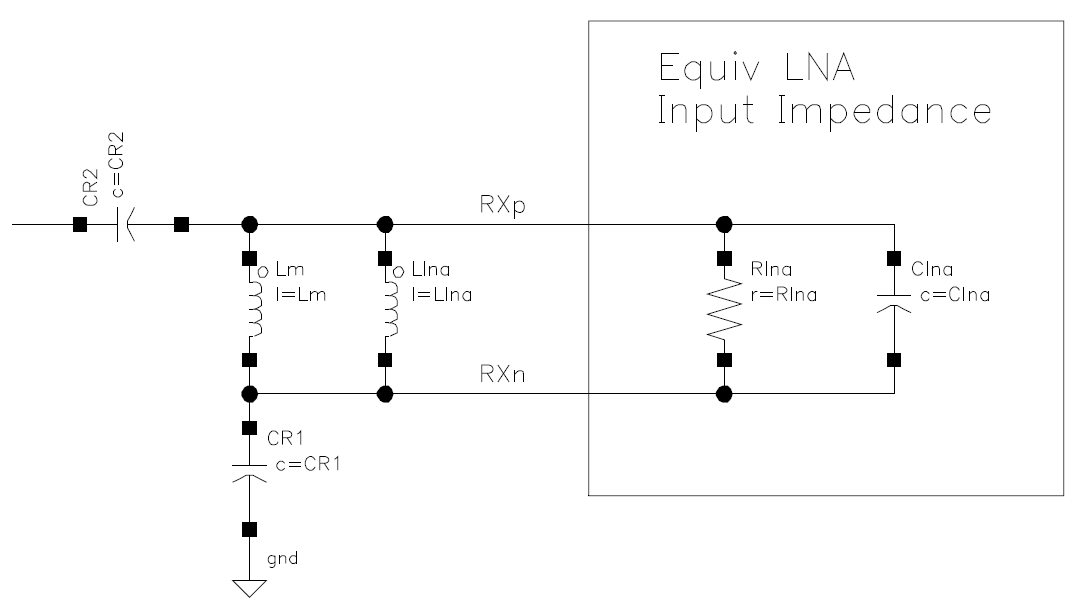
\includegraphics[width=1\linewidth]{spirit14_AN732.png}
          \caption{Resolving LR1 into Two Parts \cite[s.~9]{AN643SiliconLabs}}
          \label{EXP001:fig_spirit14}
        \end{figure}
        
        The values of these two inductances have previously been determined to be LLNA = 115.83 nH 
        and LM = 55.12 nH. As the inductance LLNA is simply used to resonate with CLNA at the 
        desired frequency of operation, the match network may thus be re-drawn as shown in Figure 
        \ref{EXP001:fig_spirit15}.

        \begin{figure}[ht!] %\ref{EXP001:fig_spirit15}
          \centering
          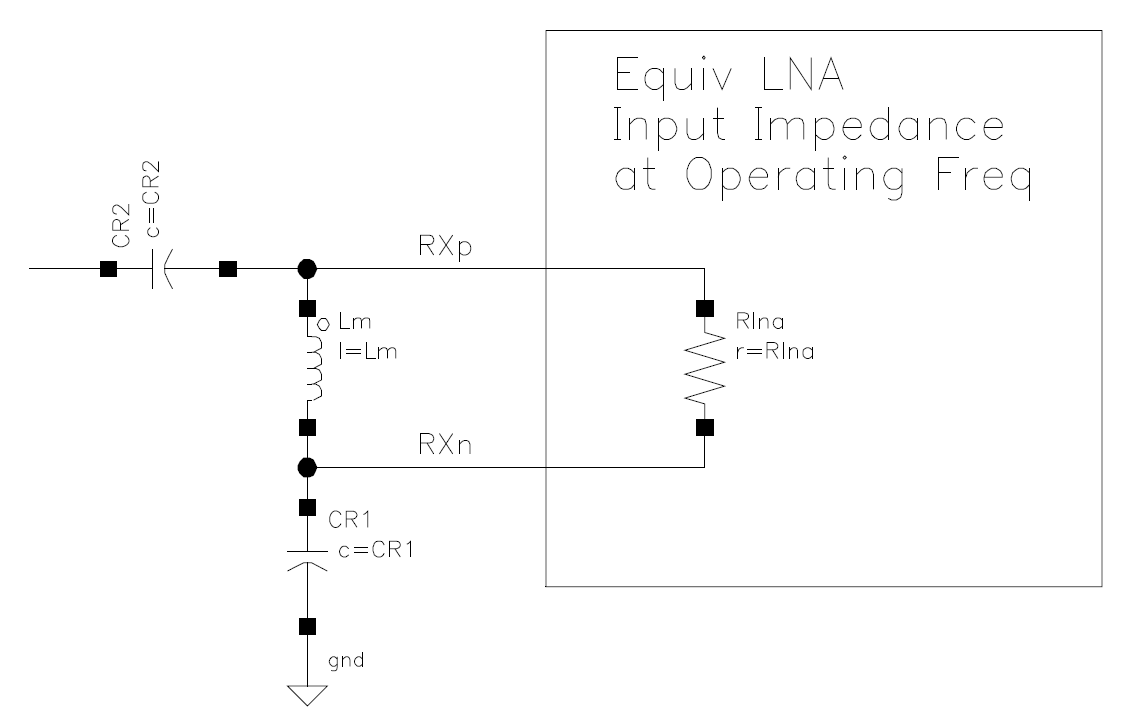
\includegraphics[width=1\linewidth]{spirit15_AN732.png}
          \caption{Equivalent Match Network at Operating Frequency \cite[s.~10]{AN643SiliconLabs}}
          \label{EXP001:fig_spirit15}
        \end{figure}
        
        The voltage across LM is desired to be twice the amplitude (and opposite in phase) to the 
        voltage across CR1. Temporarily ignoring the effects of R LNA , the following relationship 
        is obtained:
        
        \begin{equation}\label{EXP001:eq_spirit16}
         X_{LM} = 2\cdot X_{CR1}
        \end{equation}
        As the required value of inductance LM has already been determined, the required value for 
        CR1 follows immediately from the previously-derived equation for LM.
        \begin{equation}\label{EXP001:eq_spirit17}
          C_{R1} = 2\cdot\frac{\sqrt{\frac{R_{LNA}}{\SI{50}{\ohm}}-1}}{\omega_0\cdot R_{LNA}}
        \end{equation}
        Using this equation, the value for this capacitor is determined to be CR1 = 4.16 pF. It is 
        then a simple matter to allocate the remaining portion of total required series capacitive 
        reactance to CR2.
        \begin{equation}\label{EXP001:eq_spirit18}
          C_{R2} = \frac{1}{\frac{1}{C_{TOTAL}-\frac{1}{C_{R1}}}}
        \end{equation}
        From this equation, the value for the remaining capacitor is quickly found to be CR2 = 5.27 
        pF. Thus all of the components in the 3-element match network have been determined:
        \begin{itemize}\addtolength{\itemsep}{-0.5\baselineskip}
          \item CR2 = 5.27 pF
          \item LR1 = 37.35 nH
          \item CR1 = 4.16 pF
        \end{itemize}
        
      \subsubsection{Phase Imbalance of RXp/RXn Signals}
        If the input impedance of the LNA were infinite (RLNA = ∞ ), this procedure would result in 
        equal-amplitude perfectly-balanced (180° out-of-phase) waveforms at the RXp and RXn nodes. 
        However, a finite value for RLNA has the effect of shifting the phase of the signal 
        developed across the parallel combination of LR1- RLNA -CLNA; thus the voltage developed at 
        the RXp node can never be exactly 180° out-of-phase with respect to the voltage at the RXn 
        node. This effect may be clearly seen in the simulated results of Figure 10; the 
        differential voltages are equal in amplitude but not quite opposite in phase.
        \begin{figure}[ht!] %\ref{EXP001:fig_spirit17}
          \centering
          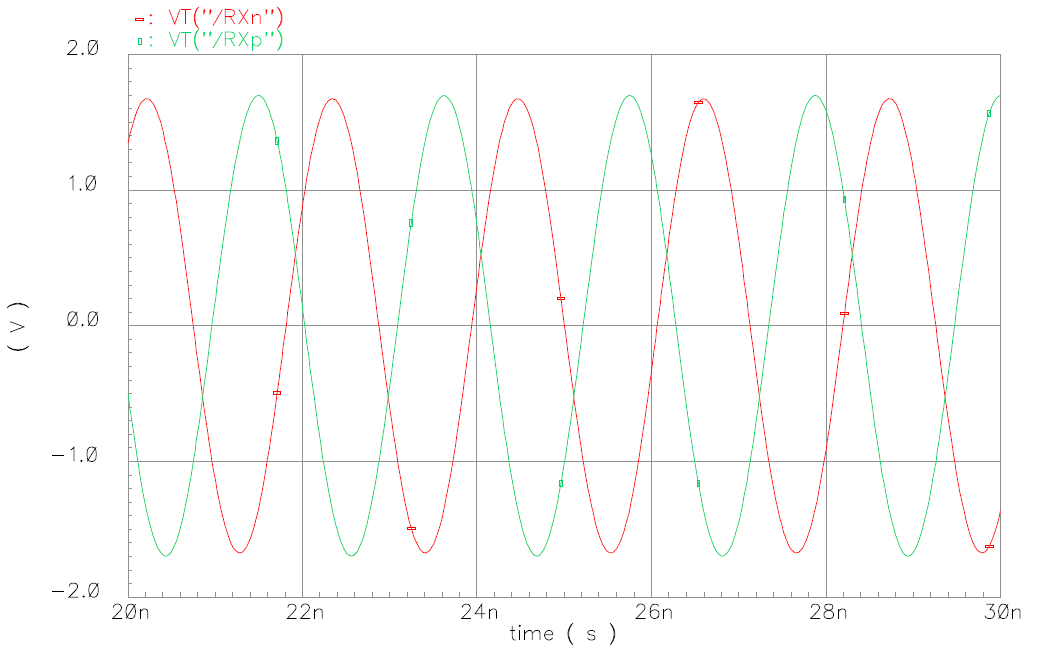
\includegraphics[width=1\linewidth]{spirit17_AN643.png}
          \caption{Differential Voltage Waveforms at LNA Input (3-Element Match) 
                  \cite[s.~11]{AN643SiliconLabs}}
          \label{EXP001:fig_spirit17}
        \end{figure}
        
        As stated earlier, the 3-element match network provides slightly less-than-optimal 
        performance when compared to a perfect balun. However, the difference is usually quite 
        small (< 0.5 dB degradation) and is often acceptable. 
        
      \subsubsection{Summary Tables of 3-Element Match Network Component Values vs. Frequency}
        Some users may not be greatly interested in the theoretical development of the matching 
        network, but are concerned only with quickly obtaining a set of component values for a 
        given desired frequency of operation. For those users, the resulting calculated component 
        values for the 3-element match network for multiple frequencies across the operating range 
        of the Si446x/Si4362 RFIC are summarized below. The calculations in this table assume the 
        ant nna source impedance is ZANT = 50 + j0Ω.
        
        The above analysis assumes use of ideal discrete components in the matching network. 
        However, surface-mount 0603- or 0402-size components themselves contain parasitic elements 
        that modify their effective values at the  frequency of interest. Additionally, the 
        analysis presented above does not make allowance for any PCB parasitics, such as trace 
        inductance, component pad capacitance, etc. Furthermore, it is convenient to use the 
        nearest available 5\% or 10\% component value; the component values shown above represent 
        results of exact mathematical calculations.
        
        As a result, it will almost certainly be necessary to “tweak” the final matching values for 
        a specific application and board layout. The above component values should be used as 
        starting points, and the values modified slightly to zero-in on the best match to the 
        antenna source impedance (e.g., 50 Ω), and the best RX sensitivity.
        
        Silicon Laboratories has empirically determined the optimum matching network values at a 
        variety of frequencies, using RF Test Boards designed by (and available from) Silicon 
        Laboratories. Wire-wound inductors (Murata LQW15A 0402-series and LQW18A 0603-series) were 
        used in all of these matching examples. Multi-layer inductors (such as Murata LQG15HS 
        0402-series) may also be used; however, the insertion loss of the match may be increased 
        slightly due to the higher loss of these inductors. By comparing the empirical values of 
        Table 3 with the calculated values of Table 2, the reader may observe that the component 
        values are in close agreement at frequencies below 500 MHz. However, somewhat larger 
        deviations in value occur at higher frequencies, primarily due to the unmodeled 
        parasitic effects of the PCB traces and discrete components. As mentioned previously, the 
        calculated matching component values of Table 2 should be used as a starting point and 
        adjusted for best performance.
        
        A 3-element RX match at 470 MHz was built and tested, using CR1=3.9 pF, LR1=39 nH, and 
        CR2=5.1 pF. The measured input impedance (S11) is shown in Figure 18.
        
        \begin{figure}[ht!] %\ref{EXP001:fig_spirit18}
          \centering
          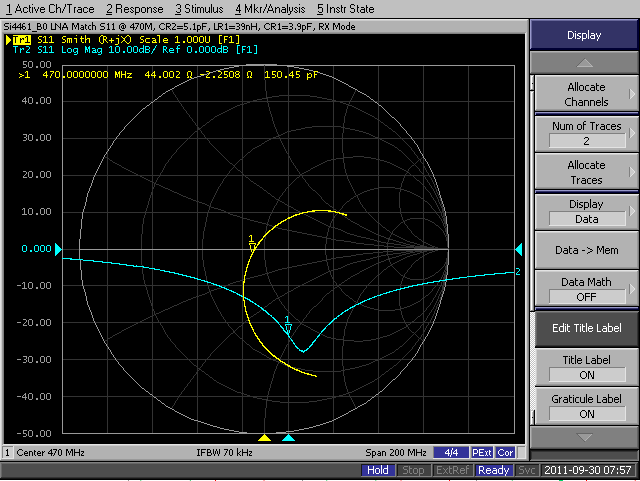
\includegraphics[width=1\linewidth]{spirit18_AN643.png}
          \caption{Input Impedance of 3-Element Match at 470 MHz \cite[s.~14]{AN643SiliconLabs}}
          \label{EXP001:fig_spirit18}
        \end{figure}
        
    \subsection{Four-Element Matching Procedure}
      As discussed previously, it is possible to achieve a theoretically-perfect match with the 
      4-element match network shown in Figure 9. The complete mathematical derivation of the 
      equations for the required component values is beyond the scope of this application note; a 
      Mathcad worksheet containing the complete derivation is available from Silicon Laboratories 
      upon request.
      
      The matching procedure for the 3-element network was readily understood and explained by 
      plotting each step on a Smith Chart. This graphical approach is somewhat less intuitive for 
      the 4-element matching procedure. Therefore, a combination of graphical and textual 
      descriptions of the main steps in the mathematical derivation is presented, along with the 
      important equations resulting from following these steps.
       
      \subsubsection{Step 1: Voltage at the RXn Node (VRXn)}
        If a network is created to successfully match to a purely-real input impedance of ZIN = 50 
        Ω, the input current IIN will also be purely real (arbitrarily assuming an input voltage 
        from the source generator VIN of unity magnitude and zero phase). This input current passes 
        through capacitor CR1 to develop the voltage at the RXn node (VRXn). It is apparent that 
        this voltage VRXn exhibits a –90° phase shift with respect to the input current IIN, due to 
        the capacitive reactance of CR1.
        
      \subsubsection{Step 2: Voltage at the RXp Node (VRXp)}
        The voltage at the RXp node (VRXp) is desired to be equal in amplitude to VRXn but opposite 
        in phase. For this condition to be satisfied, the voltage across the LNA input pins must be 
        twice the amplitude of VRXn, as well as exactly opposite in phase. That is to say, if the 
        phase of VRXn is –90°, the phase of VRXp must be +90°.
        
      \subsubsection{Step 3: Splitting the Input Current}
        Although the phase of the voltage across the LNA input pins must be +90°, the input 
        impedance of the LNA network is not purely inductive (unless RLNA = ∞). Thus, for the 
        voltage across the LNA network to be purely reactive, the phase of the current through the 
        LNA network must compensate for the phase shift introduced by RLNA. As a result, it is 
        necessary that the current through the LNA network be different from the current through 
        CR1.
        
        Thus the purpose of inductor LR2 is to split the input current IIN into two different 
        components, with the current passing through the LNA network being of the appropriate phase 
        to produce a voltage of opposite phase to VRXn.
        
        \begin{align}
          L_{R2}  &= \frac{\sqrt{\Re{Z_{ANT}}\cdot R_{LNA}}}{\omega_0} 
                   = \frac{\sqrt{\SI{50}{\ohm}\cdot R_{LNA}}}{\omega_0} 
                   \label{EXP001:eq_spirit20}   \\ 
          C_{R2}  &= \frac{1}{\omega_0^2\cdot L_{R2}}          \label{EXP001:eq_spirit21}   \\ 
          C_{R1}  &= 2\cdot C_{R2}                             \label{EXP001:eq_spirit22}   \\ 
          L_{LNA} &= \frac{1}{\omega_0^2\cdot C_{LNA}}         \label{EXP001:eq_spirit23}   \\ 
          L_{M}   &= 2\cdot L_{R2}                             \label{EXP001:eq_spirit24}   \\ 
          L_{R1}  &= \frac{L_{LNA}\cdot L_M}{L_{LNA} + L_M}    \label{EXP001:eq_spirit25}   \\ 
        \end{align}
        Continuing the design example at 470 MHz, the component values for a 4-element match 
        network are calculated as follows:
        \begin{itemize}\addtolength{\itemsep}{-0.5\baselineskip}
          \item CR1 = 4.40 pF
          \item LR1 = 54.87 nH
          \item CR2 = 2.20 pF
          \item LR2 = 52.13 nH          
        \end{itemize}
        
      \subsubsection{Phase Balance of RXp/RXn Signals}
        It was previously stated that an advantage of the 4-element match network was the ability 
        to achieve perfect phase balance (180 degrees) between the RXp and RXn input nodes. This 
        effect may be clearly seen in Figure 19; the differential voltages are now both equal in 
        amplitude and perfectly opposite in phase.
        
        \begin{figure}[ht!] %\ref{EXP001:fig_spirit16}
          \centering
          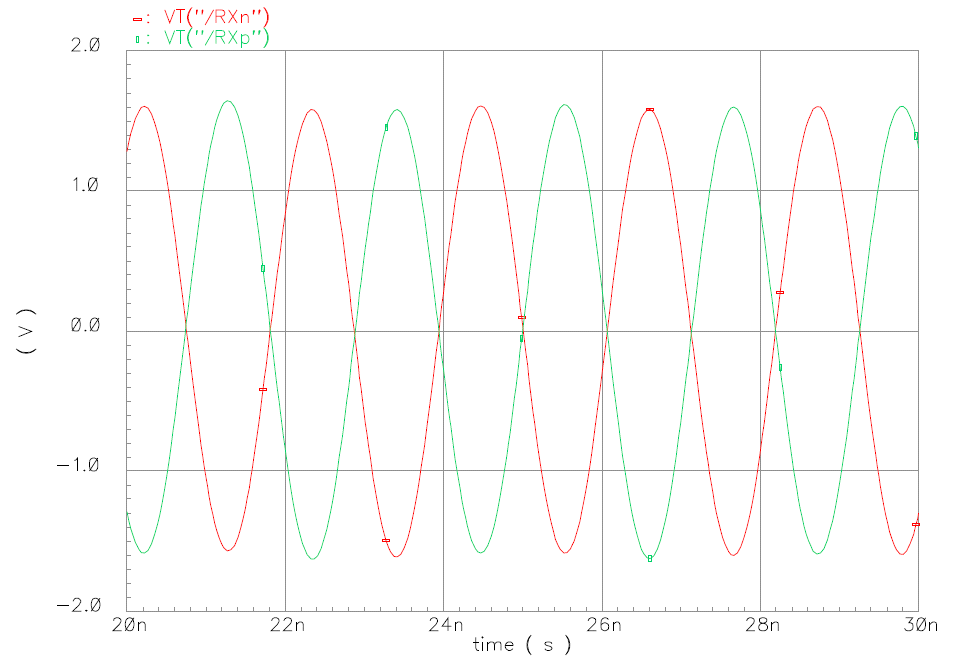
\includegraphics[width=1\linewidth]{spirit16_AN643.png}
          \caption{Differential Voltage Waveforms at LNA Input (4-Element Match) 
                   \cite[s.~16]{AN643SiliconLabs}}
          \label{EXP001:fig_spirit16}
        \end{figure}
        
      \subsubsection{Graphical Interpretation of 4-Element Match}
        It is informative to consider a graphical interpretation of the 4-element match using a 
        Smith Chart. In practicality, it is simpler to use the design equations to obtain the 
        required component values. However, the reader may gain insight into the behavior and 
        functionality of the match by tracing its impedance progression on a Smith Chart. The 
        investigation is simplified if the LNA input impedance is temporarily considered to be 
        purely real (i.e., CLNA = 0 pF). Although this situation does not exist in practice, the 
        input capacitance of the LNA may be easily canceled at the desired frequency of 
        operation by placing a parallel inductance LLNA across the RXp/RXn input pins, as discussed 
        in "4.1.2. Step 2: Add Parallel Inductance LLNA to Resonate with LNA Capacitance" on page 
        6. After cancellation of the input capacitance CLNA, the “starting” point on the Smith 
        Chart for the matching procedure then becomes ZLNA = RLNA + j0 = RLNA.
        
        If considering only the input impedance (while ignoring differential signal balance), the 
        entire match circuitry may be redrawn as shown in Figure 13. While this schematic does not 
        represent the physical arrangement of components of the match, its input impedance is 
        identical to that of the actual circuit. Furthermore, representation of the match network 
        in this “ladder” form simplifies plotting the progression of the impedance match on a Smith 
        Chart.
        
        \begin{figure}[ht!] %\ref{EXP001:fig_spirit19}
          \centering
          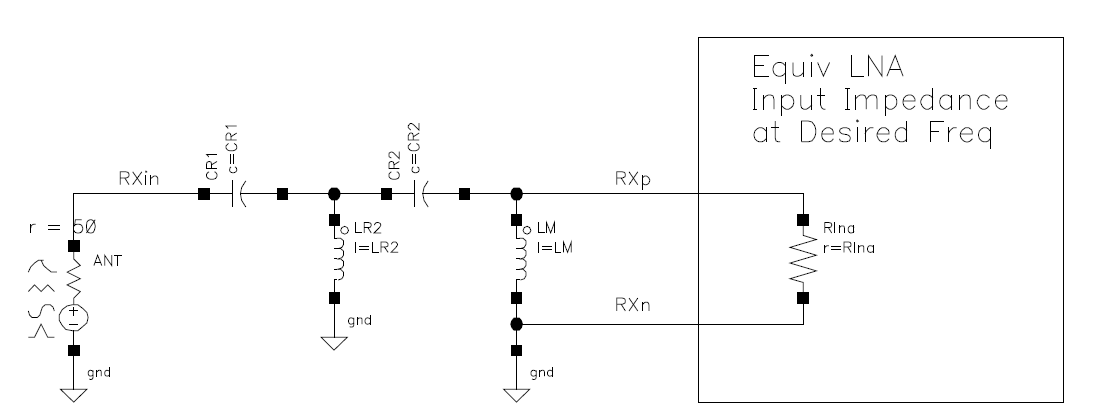
\includegraphics[width=1\linewidth]{spirit19_AN643.png}
          \caption{4-Element Match (re-drawn in ladder form) \cite[s.~17]{AN643SiliconLabs}}
          \label{EXP001:fig_spirit19}
        \end{figure}
        
        Equation \ref{EXP001:eq_spirit20} may be manipulated as follows:
        \begin{equation}\label{EXP001:eq_spirit26}
          X_{LR2} = \omega_0\cdot L_{R2} 
                  = \sqrt{\Re{Z_{ANT}\cdot R_{LNA}}} 
                  = \sqrt{\SI{50}{\ohm}\cdot R_{LNA}}
        \end{equation}
        
        This equation states that the inductive reactance of LR2 is equal to the geometric mean of 
        the antenna source impedance (e.g., 50 Ω) and the real part of the LNA input impedance 
        RLNA. Equation 9 states that the reactance of CR2 is equal to the reactance of LR2 (i.e., 
        together they resonate at the desired frequency of operation). Equation 12 then further 
        indicates that the matching inductor LM is equal to 2 x LR2, while indicates that CR1 is 
        equal to 2 x CR2.
        
        It is informative to consider the Q-factors formed by RLNA in parallel with LM, and by CR1 
        in series with RANT.
        
        \begin{align}
          Q_{LNA} &= \frac{R_{LNA}}{X_{LM}} 
                   = \frac{R_{LNA}}{\omega_0\cdot L_{M}}    \nonumber \\
                  &= \frac{R_{LNA}}{2\omega_0\cdot L_{R2}} 
                   = \frac{R_{LNA}}{2\sqrt{\SI{50}{\ohm}\cdot R_{LNA}}}
                   = \sqrt[0,5]{\frac{R_{LNA}}{\SI{50}{\ohm}}}        \label{EXP001:eq_spirit27} \\ 
          Q_{ANT} &= \frac{X_{CR1}}{R_{ANT}} 
                   = \frac{X_{CR2}}{2\cdot R_{ANT}}         \nonumber \\
                  &= \frac{X_{LR2}}{2\cdot R_{ANT}} 
                   = \frac{\sqrt{\SI{50}{\ohm}\cdot R_{LNA}}}{2\cdot \SI{50}{\ohm}}
                   = \sqrt[\frac{1}{2}]{\frac{R_{LNA}}{\SI{50}{\ohm}}}  \label{EXP001:eq_spirit28}  
        \end{align}
        
        It is well known that the locus of all impedance points with the same Q-factor describes an 
        ellipse on a Smith Chart. These last two equations indicate that the impedance at two of 
        the internal nodes within the 4-element match share the same Q-factor and thus fall upon 
        the same ellipse (constant-Q curve) on a Smith Chart. This is illustrated in the impedance 
        progression plot of 
        \ref{EXP001:fig_spirit20}.
        
        \begin{figure}[ht!] %\ref{EXP001:fig_spirit20}
          \centering
          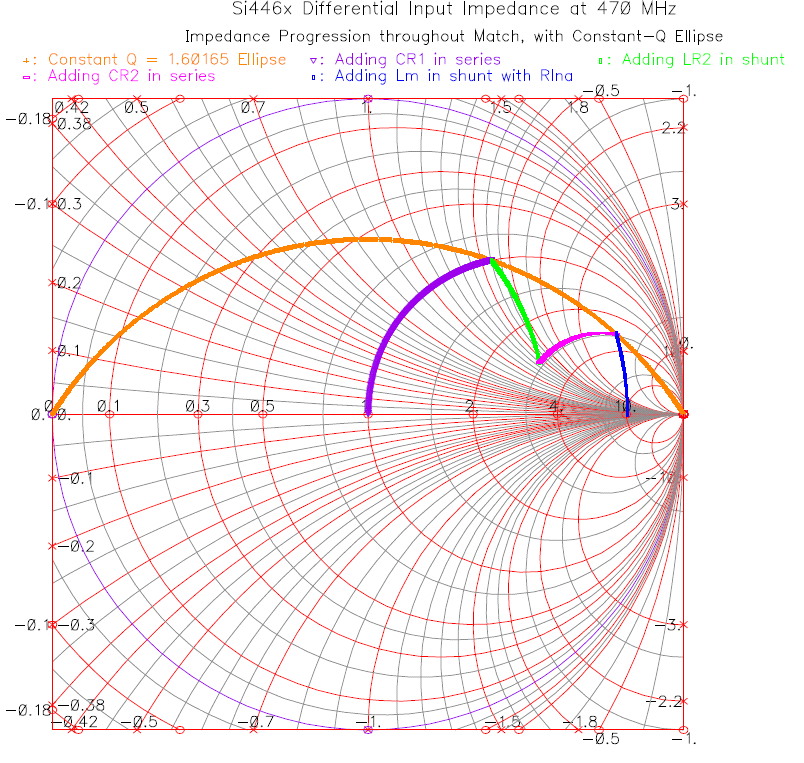
\includegraphics[width=1\linewidth]{spirit20_AN643.png}
          \caption{Impedance Match Progression Plot (with constant-Q Ellipse) \cite[s.~18]{AN643SiliconLabs}}
          \label{EXP001:fig_spirit20}
        \end{figure}
        
        In this plot, the impedance path on the Smith Chart is traced as each successive component 
        in the match is added. The plot begins on the purely-real axis at Z = RLNA + j0. The dark 
        blue curve describes the change in impedance as the matching inductor LM is added in 
        parallel with RLNA, the pink curve describes subsequently adding on series capacitor CR2, 
        and so on. Using the component values in the design example at 470 MHz, the calculated LNA 
        Q value is ~1.6 as shown in Equation 
        \ref{EXP001:eq_spirit29}.
        \begin{equation}\label{EXP001:eq_spirit29}
          Q_{LNA} = \sqrt[\frac{1}{2}]{\frac{R_{LNA}}{\SI{50}{\ohm}}}
                  = \sqrt[\frac{1}{2}]{\frac{\SI{513}{\ohm}}{\SI{50}{\ohm}}}
                  = 1,60165
        \end{equation}
        
        As predicted in the earlier discussion, it is found that the endpoints of two of the 
        segments in this impedance progression plot fall directly upon the Q = 1.60165 elliptical 
        curve.
        
        This then suggests a graphical solution to the problem of constructing a 4-element match network:
        \begin{itemize}\addtolength{\itemsep}{-0.5\baselineskip}
          \item Plot both RLNA and RANT on the Smith Chart
          \item Calculate \(Q_{LNA} = \sqrt[\frac{1}{2}]{\frac{R_{LNA}}{\SI{50}{\ohm}}}\)
          \item Construct a constant-Q ellipse on the Smith Chart with this value of Q
          \item Plot the intersection of the constant-RANT impedance circle (e.g., 50 circle) with 
                this ellipse
          \item Plot the intersection of the constant-GLNA admittance circle with this ellipse
          \item These four points (RANT, RLNA, two Q-intersection points) describe four of the 
                five segment endpoints of the impedance progression plot
          \item The fifth endpoint is graphically obtained from the segments (series CR2, shunt  
                LR2) that must be traversed to connect the two constant-Q points.
        \end{itemize}
        The corresponding component values are readily obtained by denormalizing each shunt or series path 
        traversed on the Smith Chart.

      \subsubsection{Summary Tables of 4-Element Match Network Component Values vs. Frequency}
        In this section, further detail is provided about modifying the Class-E match for a Direct 
        Tie board configuration. A supply voltage of VDD = 3.3 V is assumed.
        
        Similar to the 3-element match network, it will almost certainly be necessary to “tweak” 
        the final matching values for a specific application and board layout due to parasitic 
        effects of PCB traces and non-ideal discrete components. The above component values should 
        be used as starting points, and the values modified slightly to zero-in on the best match 
        to the antenna source impedance (e.g., 50 Ω), and the best RX sensitivity. 
        
        Silicon Laboratories has empirically determined the optimum matching network values at a 
        variety of frequencies, using RF Test Boards designed by (and available from) Silicon 
        Laboratories. Wire-wound inductors (Murata LQW15A 0402-series and LQW18A 0603-series) were 
        used in all of these matching examples. Multi-layer inductors (such as Murata LQG15HS 
        0402-series) may also be used; however, the insertion loss of the match may be increased 
        slightly due to the higher loss of these inductors. By comparing the empirical values of 
        Table 5 with the calculated values of Table 4, the reader may observe that the component 
        values are in close agreement at frequencies below 500 MHz. However, somewhat larger 
        deviations in value occur at higher frequencies, primarily due to the unmodeled 
        parasitic effects of the PCB traces and discrete components. As mentioned previously, the 
        calculated matching component values of Table 4 should be used as a starting point and 
        adjusted for best performance.
        
        A 4-element RX match at 470 MHz was built and tested, using CR1=3.9pF, LR1=56nH, CR2=2.2pF, 
        and LR2=51nH. The measured input impedance (S11) is shown in Figure 15.

        \begin{figure}[ht!] %\ref{EXP001:fig_spirit21}
          \centering
          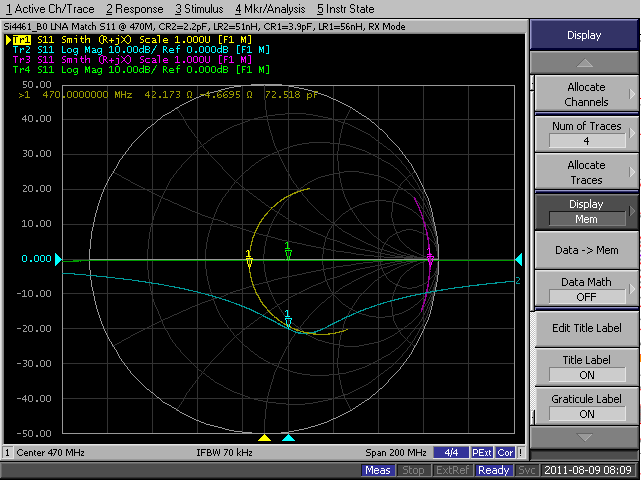
\includegraphics[width=1\linewidth]{spirit21_AN643.png}
          \caption{Input Impedance of 4-Element Match at 470 MHz \cite[s.~21]{AN643SiliconLabs}}
          \label{EXP001:fig_spirit21}
        \end{figure}
        
  \section{Modification of Class-E Match for Direct Tie Board Configuration}
    \subsection{Concept of Direct Tie Matching}
      In the Direct Tie board configuration, the TX and RX paths are tied directly together at a 
      common point without the use of an RF switch. Careful design procedure must be followed to 
      ensure that the RX input circuitry does not load down the TX output path while in TX mode, 
      and that the TX output circuitry does not degrade receive performance while in RX mode.
      
      The RX input circuitry of the Si4438 chip contains a set of switches that aids in isolation 
      of the TX and RX functions. This set of switches is implemented internally as shown in Figure 
      \ref{EXP001:fig_spirit04}.
    
      \begin{figure}[ht!]  % \ref{EXP001:fig_spirit04}
        \centering
        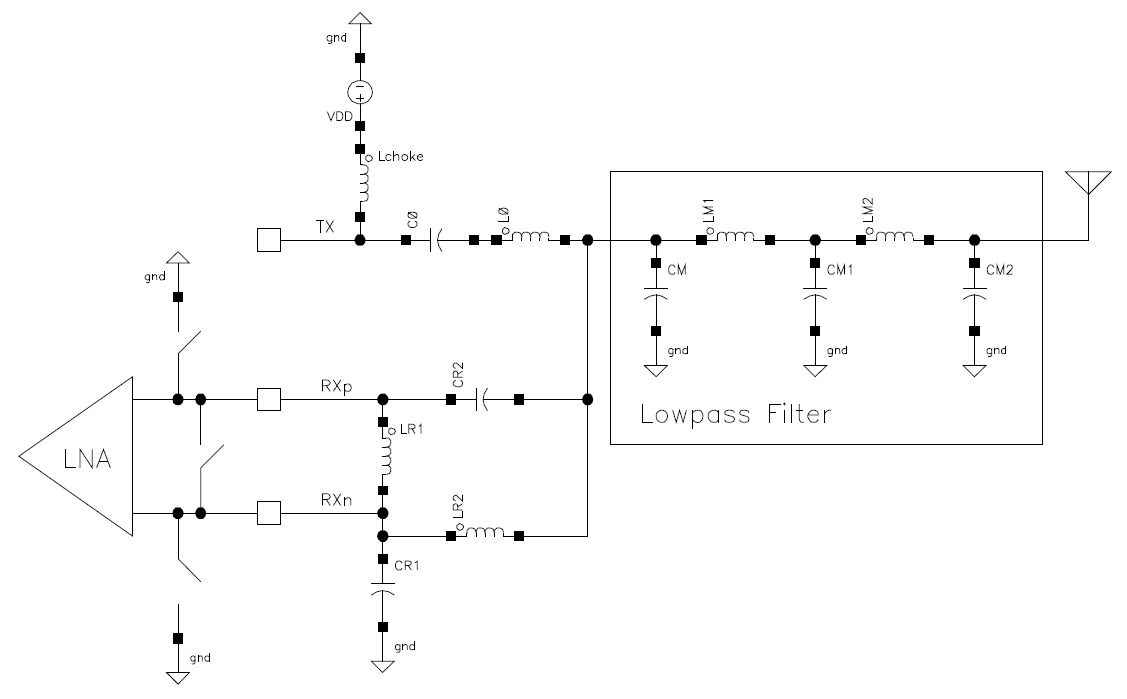
\includegraphics[width=1\linewidth]{spirit04_AN732.png}
        \caption{RX Input Switches for Direct Tie Operation \cite[s.~19]{AN648SiliconLabs}}
        \label{EXP001:fig_spirit04}
      \end{figure}
      
      These three switches are activated and closed simultaneously upon entering TX mode; the 
      switches remain open in all other modes, including RX mode. Closing these switches during TX 
      mode effectively shorts the RXp and RXn input pins together and also shorts them to GND. The 
      effective circuit may be re-drawn as shown in Figure \ref{EXP001:fig_spirit05}. Inductor LR2 
      and capacitor CR2 have effectively been placed in parallel by the closure of the switches, 
      and are connected to GND. If the values of these components are chosen for resonance at the 
      desired operating frequency, a very high impedance is presented to the TX path resulting in 
      very little degradation in TX output power. Also, by shorting the input pins of the LNA 
      together and simultaneously to GND, the LNA is protected from the large signal swing of the 
      TX signal. This feature allows connection of the TX path to the RX path without damage to the 
      LNA.
      \begin{figure}[ht!]  % \ref{EXP001:fig_spirit05}
        \centering
        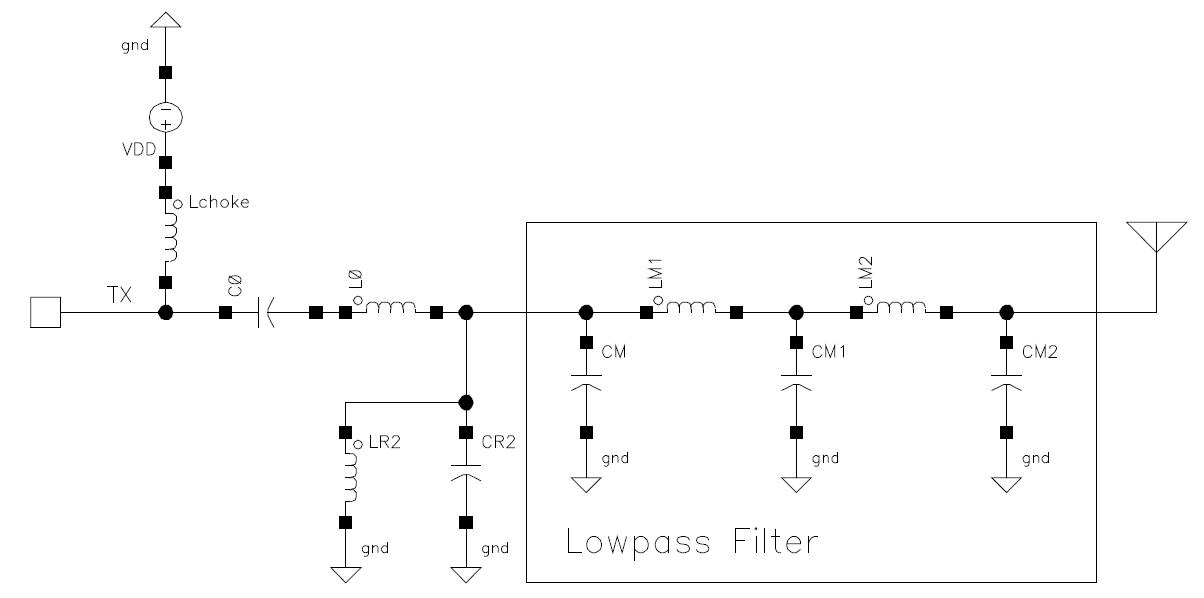
\includegraphics[width=1\linewidth]{spirit05_AN732.png}
        \caption{Effective Class-E Direct Tie Circuit in \textbf{TX Mode}  
                 \cite[s.~20]{AN648SiliconLabs}}
        \label{EXP001:fig_spirit05}
      \end{figure}
      
      In RX mode, the output transistors of the PA are in the OFF state and the impedance seen 
      looking back into the TX pin is comprised mostly of the output capacitance of the 
      transistors. (The impedance of the pull-up inductor LCHOKE is quite high and may be ignored 
      for this discussion.) This output capacitance is effectively in series with matching 
      capacitor C0 and will result in series-resonance with inductor L0 at some frequency, as shown 
      in Figure \ref{EXP001:fig_spirit06}. At this series-resonant frequency, the input to the LNA 
      matching network is effectively shorted to GND and thus significantly degrades receive 
      performance. As the PA output capacitance CPAOFF is fixed, it is necessary to choose L0 and 
      C0 to ensure that this series-resonance does not excessively degrade RX performance at the 
      desired operating frequency. It may be necessary to alter the values of L0 and/or C0 slightly 
      away from their calculated optimum values in order to accomplish this goal, thus slightly 
      degrading TX performance in an effort to minimize the impact to RX performance.
      
      \begin{figure}[ht!]  % \ref{EXP001:fig_spirit06}
        \centering
        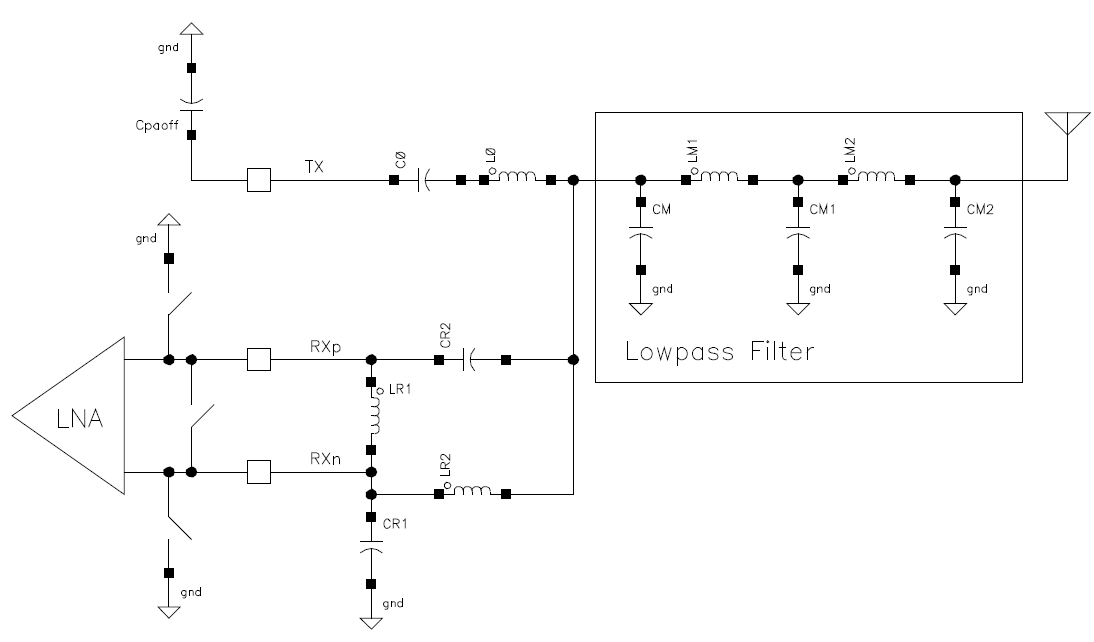
\includegraphics[width=1\linewidth]{spirit06_AN732.png}
        \caption{Effective Class-E Direct Tie Circuit in \textbf{RX Mode}}
        \label{EXP001:fig_spirit06}
      \end{figure}

  \newpage
  \section{RF konektory pro koaxiální kabely}
    \subsection{Konektor typu N}
      Konektorem \textbf{typu N} (obr.\ref{EXP001:fig_Ncon}), byl vůbec první konektor určený pro 
      koaxiální kabel umožňující přenášet mikrovlnné signály. Tento konektor byl zaveden americkým 
      inženýrem Paulem Neillem v Bellových laboratořích kolem roku 1940, po kterém je i pojmenován. 
      Pro svojí robustnost, byl původně určen pro signály do \SI{1}{\giga\hertz} ve vojenských 
      aplikaci, ale v dnešní době běžně zvládá signály o frekvencích okolo \SI{11}{\giga\hertz}. 
      Konektor se vyrábí s impedancí \SI{50}{\ohm} a \SI{70}{\ohm}.
      
      \begin{figure}[ht!]    %\ref{EXP001:fig_Ncon}
        \centering  
        \begin{tabular}{cc}
          \subfloat[Female SMA]{\label{EXP001:fig_Nmale}
            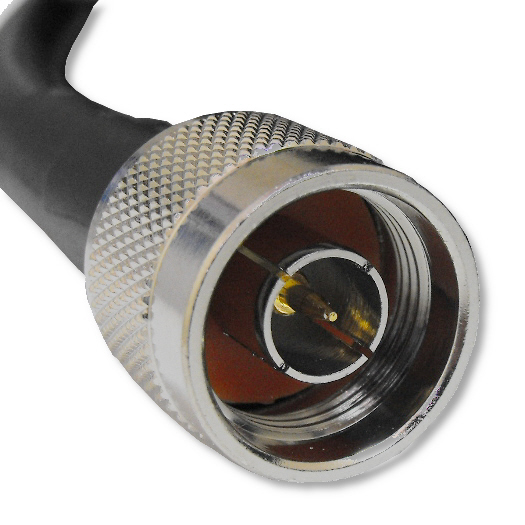
\includegraphics[width=0.2\linewidth]{con_Nmale.jpg}}              &
          \subfloat[Male SMA]{\label{EXP001:fig_Nfemale}
            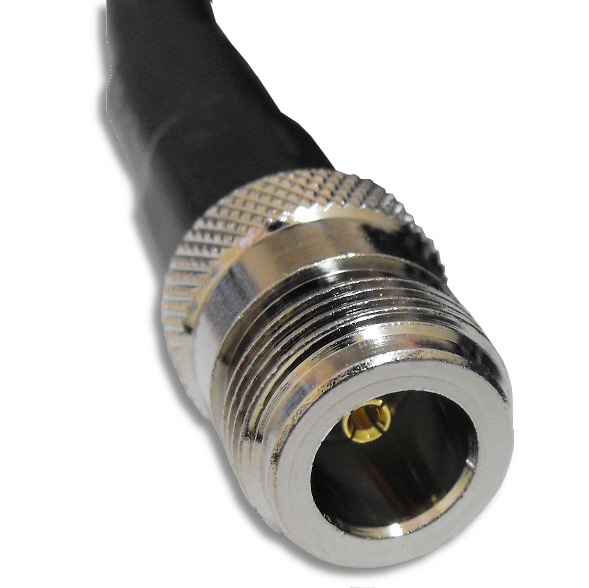
\includegraphics[width=0.2\linewidth]{con_Nfemale.jpg}}
        \end{tabular}
        \caption{Provedení konektoru typu \textbf{N}}
        \label{EXP001:fig_Ncon}
      \end{figure} 
      
    \subsection{Konektor typu SMA}
      Konektor \textbf{typu SMA} (\textbf{S}ub\textbf{M}iniature version \textbf{A}), byl navrhnut 
      v roce 1960. Jedná se o minimalistickou variantu konektoru se šroubovacím mechanismem, 
      dimenzovaným až pro 500 spojovacích cyklů. Použití ve zhoršených klimatických podmínkách se 
      nedoporučuje. Konektor má impedanci \SI{50}{\ohm} a je možné jím přenášet signály do 
      frekvence \SI{18}{\giga\hertz}.

      \begin{wrapfigure}[12]{r}{5cm}   %\ref{ES:fig_amp_law}
        \centering
        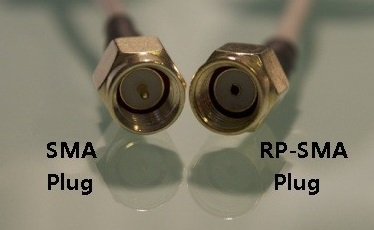
\includegraphics[width=0.9\linewidth]{SMA_RPSMA.jpg}
        \caption{Konektor SMA male (vlevo) a jeho varianta s reverzní polaritou (vpravo)}
        \label{EXP001:fig_SMA_RPSMA}
      \end{wrapfigure}
      K tomuto konektoru existuje ješte \emph{reverzní varianta} označovaná jako \textbf{RP-SMA}, 
      která je také příčinou snadné záměny těchto konektorů, jak ukazuje obrázek 
      \ref{EXP001:fig_SMA_RPSMA}. Varianta konektoru \texttt{RP-SMA} obrací polaritu rozhraní, což 
      napovídá sama zkratka: \textbf{R}everse \textbf{P}olarity \texttt{SMA}. Termín 
      "přepólování" zde v podstatě znamená změnu "pohlaví" viz obr. \ref{EXP001:fig_SMA}. Důvodem 
      zavedení této varianty byl požadavek z dob uvádění \texttt{WIFI} zařízení na trh, kdy bylo 
      nutné uživateli znemožnit připojení k zařízení běžně dostupných antén, které měli vyšší zisk, 
      čímž by docházelo k porušování podmínek pro jejich provoz v rámci daných legislativních 
      norem. Tento typ konektoru je i v roce 2014 výrobci \texttt{WIFI} zařízení stále používán, 
      ačkoliv na trhu jsou dostupné redukce.           

            
      \begin{figure}[ht!]
        \centering  
        \begin{tabular}{cccc}
          \subfloat[SMA Female]{\label{EXP001:fig_SMAf}
            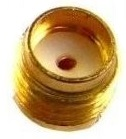
\includegraphics[width=0.2\linewidth]{SMA_female.jpg}}             &
          \subfloat[SMA Male]{\label{EXP001:fig_SMAm}
            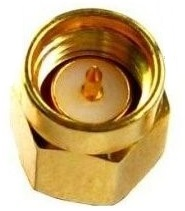
\includegraphics[width=0.2\linewidth]{SMA_male.jpg}}               &
          \subfloat[RP-SMA Female/Jack (\emph{Buchse})]{\label{EXP001:fig_RPSMAf}
            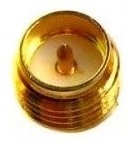
\includegraphics[width=0.2\linewidth]{RPSMA_female.jpg}}           &
          \subfloat[RP-SMA Male/Plug (\emph{Stecker})]{\label{EXP001:fig_RPSMAm}
            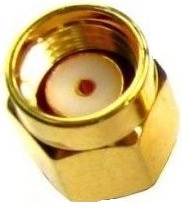
\includegraphics[width=0.2\linewidth]{RPSMA_male.jpg}}             
        \end{tabular}
        \caption{ Samička konektoru \texttt{RP-SMA} má stejný tvar vnějšího těla jako samička 
                 \texttt{SMA} konektoru, ale má vnitřní mužský pinový kontakt (Center Pin). Podobně 
                 sameček konektoru typu \texttt{RP-SMA} má místo vnitřního pinového kontaktu, 
                 zásuvku (Center Receptacle).}
        \label{EXP001:fig_SMA}
      \end{figure}  
      
  \section{Varianta 1: 433 MHz}
    \begin{figure*}[ht!]
      \centering
      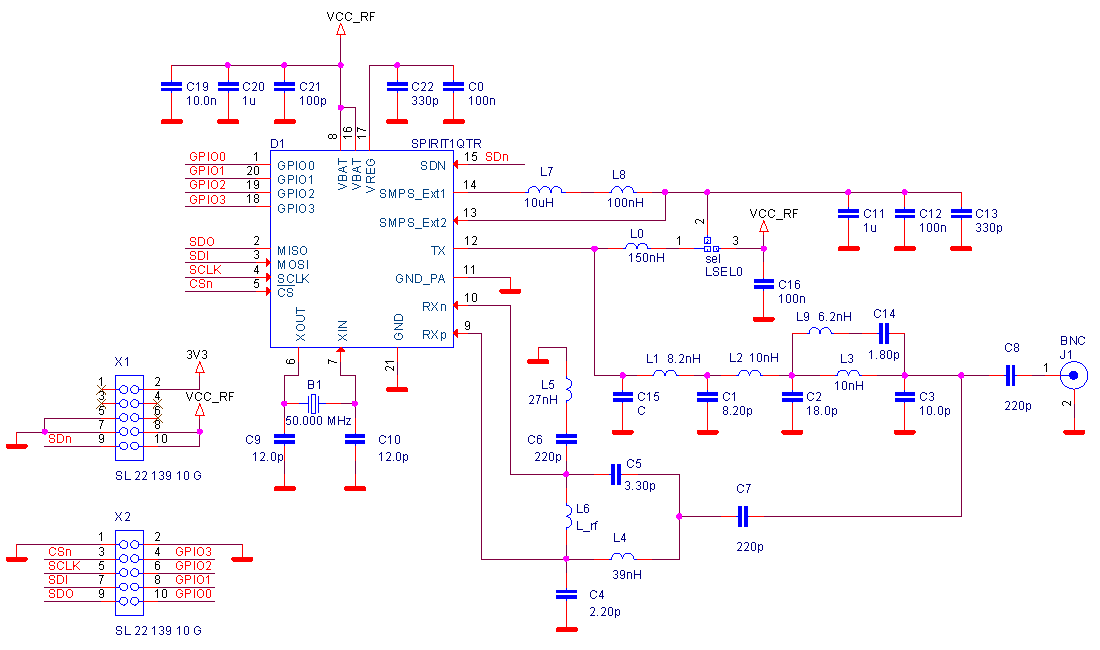
\includegraphics[width=0.9\textwidth]{modul_spirit1_sch.pdf}
      \caption{Schéma zapojení}
      \label{EXP001:fig_exp_sch434MHz}
    \end{figure*}
    
\printbibliography[heading=subbibliography]
